\documentclass[
	12pt,twoside,a4paper
]{report}

\usepackage{graphicx}
\usepackage[margin=1in]{geometry}
\usepackage{fancyhdr}
\usepackage[utf8]{inputenc}
\usepackage{etoc}
\usepackage{xcolor, soul}
\usepackage{listings}
\usepackage{amsmath}
\usepackage{lipsum}
\usepackage{pgfplots}
\usepackage{hyperref}
\usepackage{circuitikz}
\usepackage{caption}
\usepackage{subcaption}
\usepackage{listings}
\usepackage{unicode-math}
\usepackage[style=apa, backend=biber]{biblatex}

\addbibresource{refs.bib}
\DeclareLanguageMapping{english}{english-apa}

\sethlcolor{yellow}

\fancypagestyle{plain}{
	\fancyhf{}
	\fancyhead[l]{Project 2}
	\fancyhead[r]{June 10, 2024}
	\fancyfoot[le, ro]{Page \thepage}
	\fancyfoot[re, lo]{ESD Capsule 2024}
	\setlength{\headheight}{15pt}
	\renewcommand{\headrulewidth}{0.2pt}
	\renewcommand{\footrulewidth}{0.2pt}
}	

\thispagestyle{plain}

\renewcommand{\etocaftertitlehook}{\thispagestyle{plain}}
\renewcommand{\etocaftertochook}{\thispagestyle{plain}}

\begin{document}
	\begin{center}
	
\includegraphics[width=0.4\textwidth]{assets/agu.png}

	\Huge
	\textbf{Project \#2}

	\vspace{0.3cm}
	\Huge
	Helmholtz Coil Analysis

	\vspace{0.8cm}
	\large
	\vspace{0.5cm}
	\LARGE
	\vspace{1.5cm}
	\textbf{}
	\vfill
	\vspace{0.8cm}
	\Large
\end{center}

\begin{tabbing}
	\hspace*{1em} \= \hspace*{10em} \= \hspace*{11em} \= \kill
	\> \textbf{Project Team:} \> \>  \\
	\> Barış DEMİRCİ \> agu@338.rocks \> \\
	\> Selin Nisa AKGÖL \> selinnisa.akgol@agu.edu.tr \> \\
	\> Hatice Kübra DURU \> haticekubra.duru@agu.edu.tr \> \\
	\> \> \> \\
	\>  June 10, 2024 \> \> \\
\end{tabbing}

	\tableofcontents

	\chapter{Abstract}

This project aims to investigate the creation and properties of a uniform magnetic field using Helmholtz coil. Helmholtz coil consist of two identical circular coils with a specific configuration designed to generate a nearly uniform magnetic field in a certain volume of space. This report covers the theoretical background, derivation of the magnetic field equations, experimental setup, simulation results, and analysis of the Helmholtz coil system in a circuit.

	\chapter{Introduction}

Obtaining a uniform magnetic field is crucial in many physical experiments and for the operation of various electrical and electronic devices. The Helmholtz coil system, consisting of two identical coils, is a common solution for producing such a field. This project explores the conditions under which the magnetic field is most uniform and provides a detailed analysis of the system.

	\chapter{Theoretical Background}

\section{Magnetic Field of a Single Circular Coil}

\begin{figure}[h]
\centering
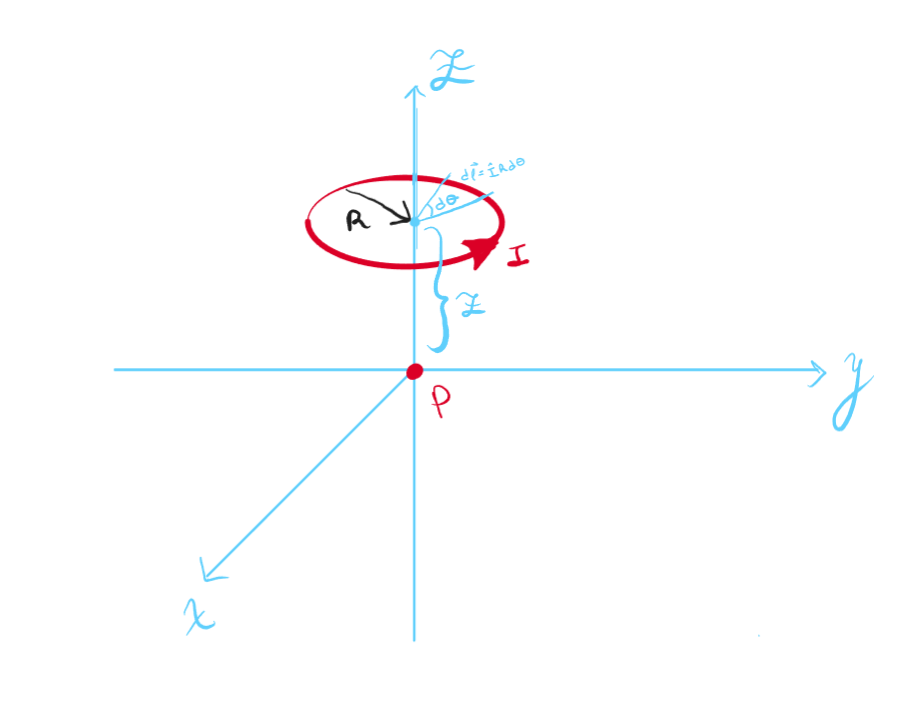
\includegraphics[width=0.5\textwidth]{assets/single-coil-magnetic-field-hand-drawn.png}
\caption{Magnetic field of a single circular coil.}
\end{figure}

The magnetic field $\vec{B}$ at point $P$ due to a current $I$ flowing through a circular coil of radius $R$ can be calculated using the Biot-Savart law:

\begin{align*} 
    d\vec{B} &= \frac{\mu_0 I}{4\pi} \frac{d\vec{l} \times \vec{r}}{|\vec{r}|^3} \\
\end{align*}

\noindent Where:
\begin{itemize}
    \item $\mu_0$ is the permeability of free space.
    \item $d\vec{l}$ is the differential length element of the coil.
    \item $\vec{r}$ is the position vector from the differential element to the point $P$.
\end{itemize}

\newpage
\thispagestyle{plain}

To find the magnetic field at point $P$ due to any radius $r$ and any arc length $l$, we can integrate the differential magnetic field over the specified arc length:

\begin{align*}
    &d\vec{l} = \hat{\theta}rd\theta \\
    &\vec{r} = -\hat{R}r -\hat{k}z \\
    &|\vec{r}| = \sqrt{r^2 + z^2} \\
    &\Rightarrow \vec{B}(r, \theta, z) = \int\limits_0^\theta d\vec{B}(r, \theta', z) \\
    &= \int\limits_0^\theta \frac{\mu_0 I r}{4\pi}\cdot(r^2 + z^2)^{-\frac{3}{2}}\cdot\left[\hat{\theta}rd\theta' \times (-\hat{R}r - \hat{k}z)\right] \\
    &\boxed{\vec{B}(r, \theta, z) = \frac{\mu_0 I r \theta}{4\pi} \cdot(r^2 + z^2)^{-\frac{3}{2}} \cdot (\hat{k}r - \hat{R}z)} \\
\end{align*}

And for a full circular coil with radius $R$ and distance from center $z$, the magnetic field is:

\begin{align*}
    \vec{B}(R, 2\pi, z) = \frac{\mu_0 I R 2\pi}{4\pi} \cdot(R^2 + z^2)^{-\frac{3}{2}} \cdot (\hat{k}R - \hat{R}z) \\
    \boxed{\vec{B}(R, 2\pi, z) = \frac{\mu_0 I R}{2} \cdot(R^2 + z^2)^{-\frac{3}{2}} \cdot (\hat{k}R - \hat{R}z)} \\
\end{align*}


\section{Magnetic Field with Coil of N Turns}

For coils with \( N \) turns, the magnetic field is simply multiplied by \( N \):

\[ \boxed{\vec{B}(R, 2\pi, z) = \frac{\mu_0 I R N}{2} \cdot(R^2 + z^2)^{-\frac{3}{2}} \cdot (\hat{k}R - \hat{R}z)} \]

\newpage{}
\thispagestyle{plain}

\section{Helmholtz Coil Configuration}

\begin{figure}[h]
    \centering  
    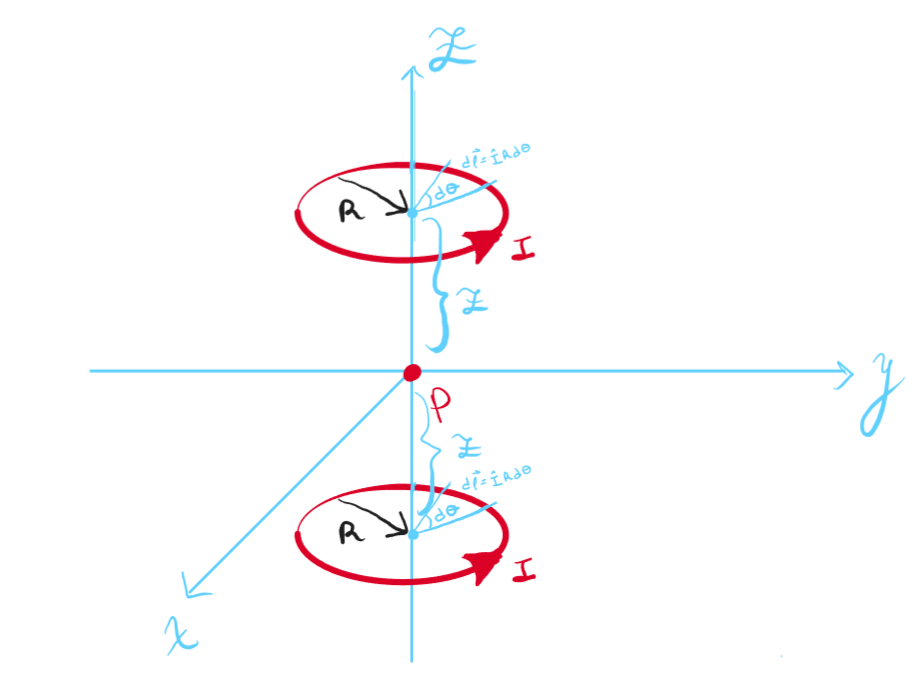
\includegraphics[width=0.5\textwidth]{assets/helmholtz-coil-setup-hand-drawn.png}
    \caption{Helmholtz coil configuration.}
    \end{figure}

For two identical coils of radius \( R \) separated by a distance \( d \) and carrying current \( I \), the magnetic field at point \( P \) is:

\begin{align*}
    \vec{B}_{\text{total}} &= \vec{B}_{\text{top}} + \vec{B}_{\text{bottom}} \\
    let~\xi(r, \theta) &= \frac{\mu_{0}Ir\theta N}{4\pi} \\
    \vec{B}_{Bottom}(r,\theta,z) &=\xi(r, \theta)\bigg[\frac{\hat{k}r+\hat{R}(z-d/2)}{(r^2+(z-d/2)^2)^{3/2}}\bigg] \\
    \vec{B}_{Top}(r,\theta,z) &=\xi(r, \theta)\bigg[\frac{\hat{k}r-\hat{R}(z+d/2)}{(r^2+(z+d/2)^2)^{3/2}}\bigg] \\
    \vec{B}_{Total}(r,\theta,z) &=\xi(r, \theta)\bigg[\frac{\hat{k}r+\hat{R}(z-d/2)}{(r^2+(z-d/2)^2)^{3/2}}+\frac{\hat{k}r-\hat{R}(z+d/2)}{(r^2+(z+d/2)^2)^{3/2}}\bigg] \\
\end{align*}

To achieve maximum uniformity at the center (\( z = 0 \)), we need to find the optimal ratio of \( d/R \).

\newpage{}
\thispagestyle{plain}

\section{Optimal Distance \( d \)}
To find the optimal distance \( d \), we need to minimize the second derivative of \( \vec{B}_{\text{total}}(R, 2\pi, z) \) at \( z = 0 \). This ensures that the magnetic field is as uniform as possible.

\begin{align*}
    \text{let}~\xi(R) &= \hat{k}2\pi \mu_0 I R^2 \\
    \vec{B}_{total}(R, 2\pi, z) &= \xi(R) \cdot \frac{1}{(R^{2}+z^{2})^{3/2}} \\
    \implies \vec{B}_{total}(R, 2\pi, \delta z) &= \xi(R) \cdot \bigg[\frac{1}{(R^{2}+(\frac{d}{2}-\delta z)^{2})^{3/2}} + \frac{1}{(R^{2}+(\frac{d}{2}+\delta z)^{2})^{3/2}}\bigg] \\ 
    \frac{\partial^{2} \vec{B}_{total}}{\partial (\delta z)^{2}} &= \xi(R) \bigg[\frac{\frac{15}{4}(d-2\delta z)^{2}}{(R^{2}+\frac{1}{4}(d-2\delta z)^{2})^{7/2}}-\frac{3}{(R^{2}+\frac{1}{4}(d-2\delta z)^{2})^{5/2}} \\ 
    &\quad -\frac{3}{(R^{2}+\frac{1}{4}(d+2\delta z)^{2})^{5/2}}+\frac{\frac{15}{4}(d-2\delta z)^{2}}{(R^{2}+\frac{1}{4}(d+2\delta z)^{2})^{7/2}}\bigg] \\ 
    \lim_{\delta z \to 0} \frac{\partial^{2} \vec{B}_{total}}{\partial (\delta z)^{2}} &= \xi(R) \bigg[\frac{\frac{15}{2}d^{2}}{(R^{2}+\frac{d^{2}}{4})^{7/2}}-\frac{6}{(R^{2}+\frac{d^{2}}{4})^{5/2}}\bigg] = 0 \\ 
    &\implies \frac{15d^{2}}{R^2+\frac{d^{2}}{4}} = 12 \\
    &\implies 15d^{2} = 12R^{2} + 3d^{2} \\
    &\implies 12d^{2} = 12R^{2} \\
    &\implies d^{2} = R^{2} \\
    &\implies d = R ~ \text{(neither $d$ nor $R$ can be negative)} \\
\end{align*}

\noindent Where:

\begin{itemize}
    \item \( d \) is the distance between the coils.
    \item \( z \) is the distance from the center of the coils.
    \item \( \delta z \) is a small change in \( z \).
    \item \( \xi(R) \) is the radius dependent coefficent.
\end{itemize}

This means that the optimal distance between the coils is equal to the radius of the coils.

\newpage{}
\thispagestyle{plain}

\section{Partial Derivatives}

\begin{align*}
    \frac{\partial \vec{B}}{\partial \theta} &= \frac{\mu_{0} Ir N}{4\pi}\Big[\frac{(\hat{k}r-\hat{R}(z+r/2))}{(r^2+(z+r/2)^2)^{3/2}}+\frac{(\hat{k}r+\hat{R}(z-r/2))}{(r^2+(z-r/2)^2)^{3/2}}\Big] \\
    \frac{\partial \vec{B}}{\partial r} &= \frac{\mu_{0} I\theta N}{4\pi}\Bigg[\frac{(2\hat{k}r-\hat{R}(2+r))}{(r^2+(z+r/2)^2)^{3/2}} -\frac{3(\hat{k}r^2 -\hat{R}(2r+r^2/2))(2r+(z+r/2))}{2(r^2+(z+r/2)^2)^{5/2}} \\
    & +\frac{(2\hat{k}r-\hat{R}(2-r))}{(r^2+(z-r/2)^2)^{3/2}}-\frac{3(\hat{k}r^2 +\hat{R}(2r-r^2/2))(2r-(z-r/2))}{2(r^2+(z-r/2)^2)^{5/2}}\Bigg] \\
    \frac{\partial \vec{B}}{\partial z} &= \frac{\mu_{0} Ir\theta N}{4\pi}\Big[\frac{-\hat{R}}{2(r^2+(z+r/2)^2)^{3/2}}-\frac{3(z+r/2)(\hat{k}r-\hat{R}(z+r/2))}{(r^2+(z+r/2)^2)^{5/2}} \\
    & -\frac{\hat{R}}{2(r^2+(z-r/2)^2)^{3/2}}-\frac{(z-r/2)(\hat{k}r+\hat{R}(z-r/2))}{3(r^2+(z-r/2)^2)^{5/2}}\Big] \\
\end{align*}

	\chapter{Experimental Setup}

\section{Coil Design}

We have designed a Helmholtz Coil on SolidWorks with a radius of $40mm$, width of $9mm$ and $30$ turns. 

\begin{figure}[h]
    \centering
    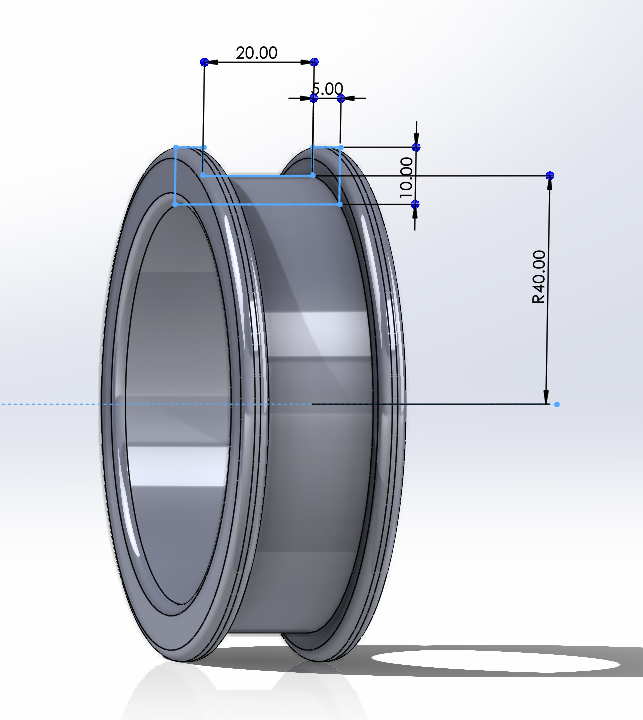
\includegraphics[width=0.4\textwidth]{assets/coil-design-single.png}
    \caption{Coil Design}
    \label{fig:helmholtz-coil}
\end{figure}

And we have 3D printed the coil design with PLA filament.

\begin{figure}[h]
    \centering
    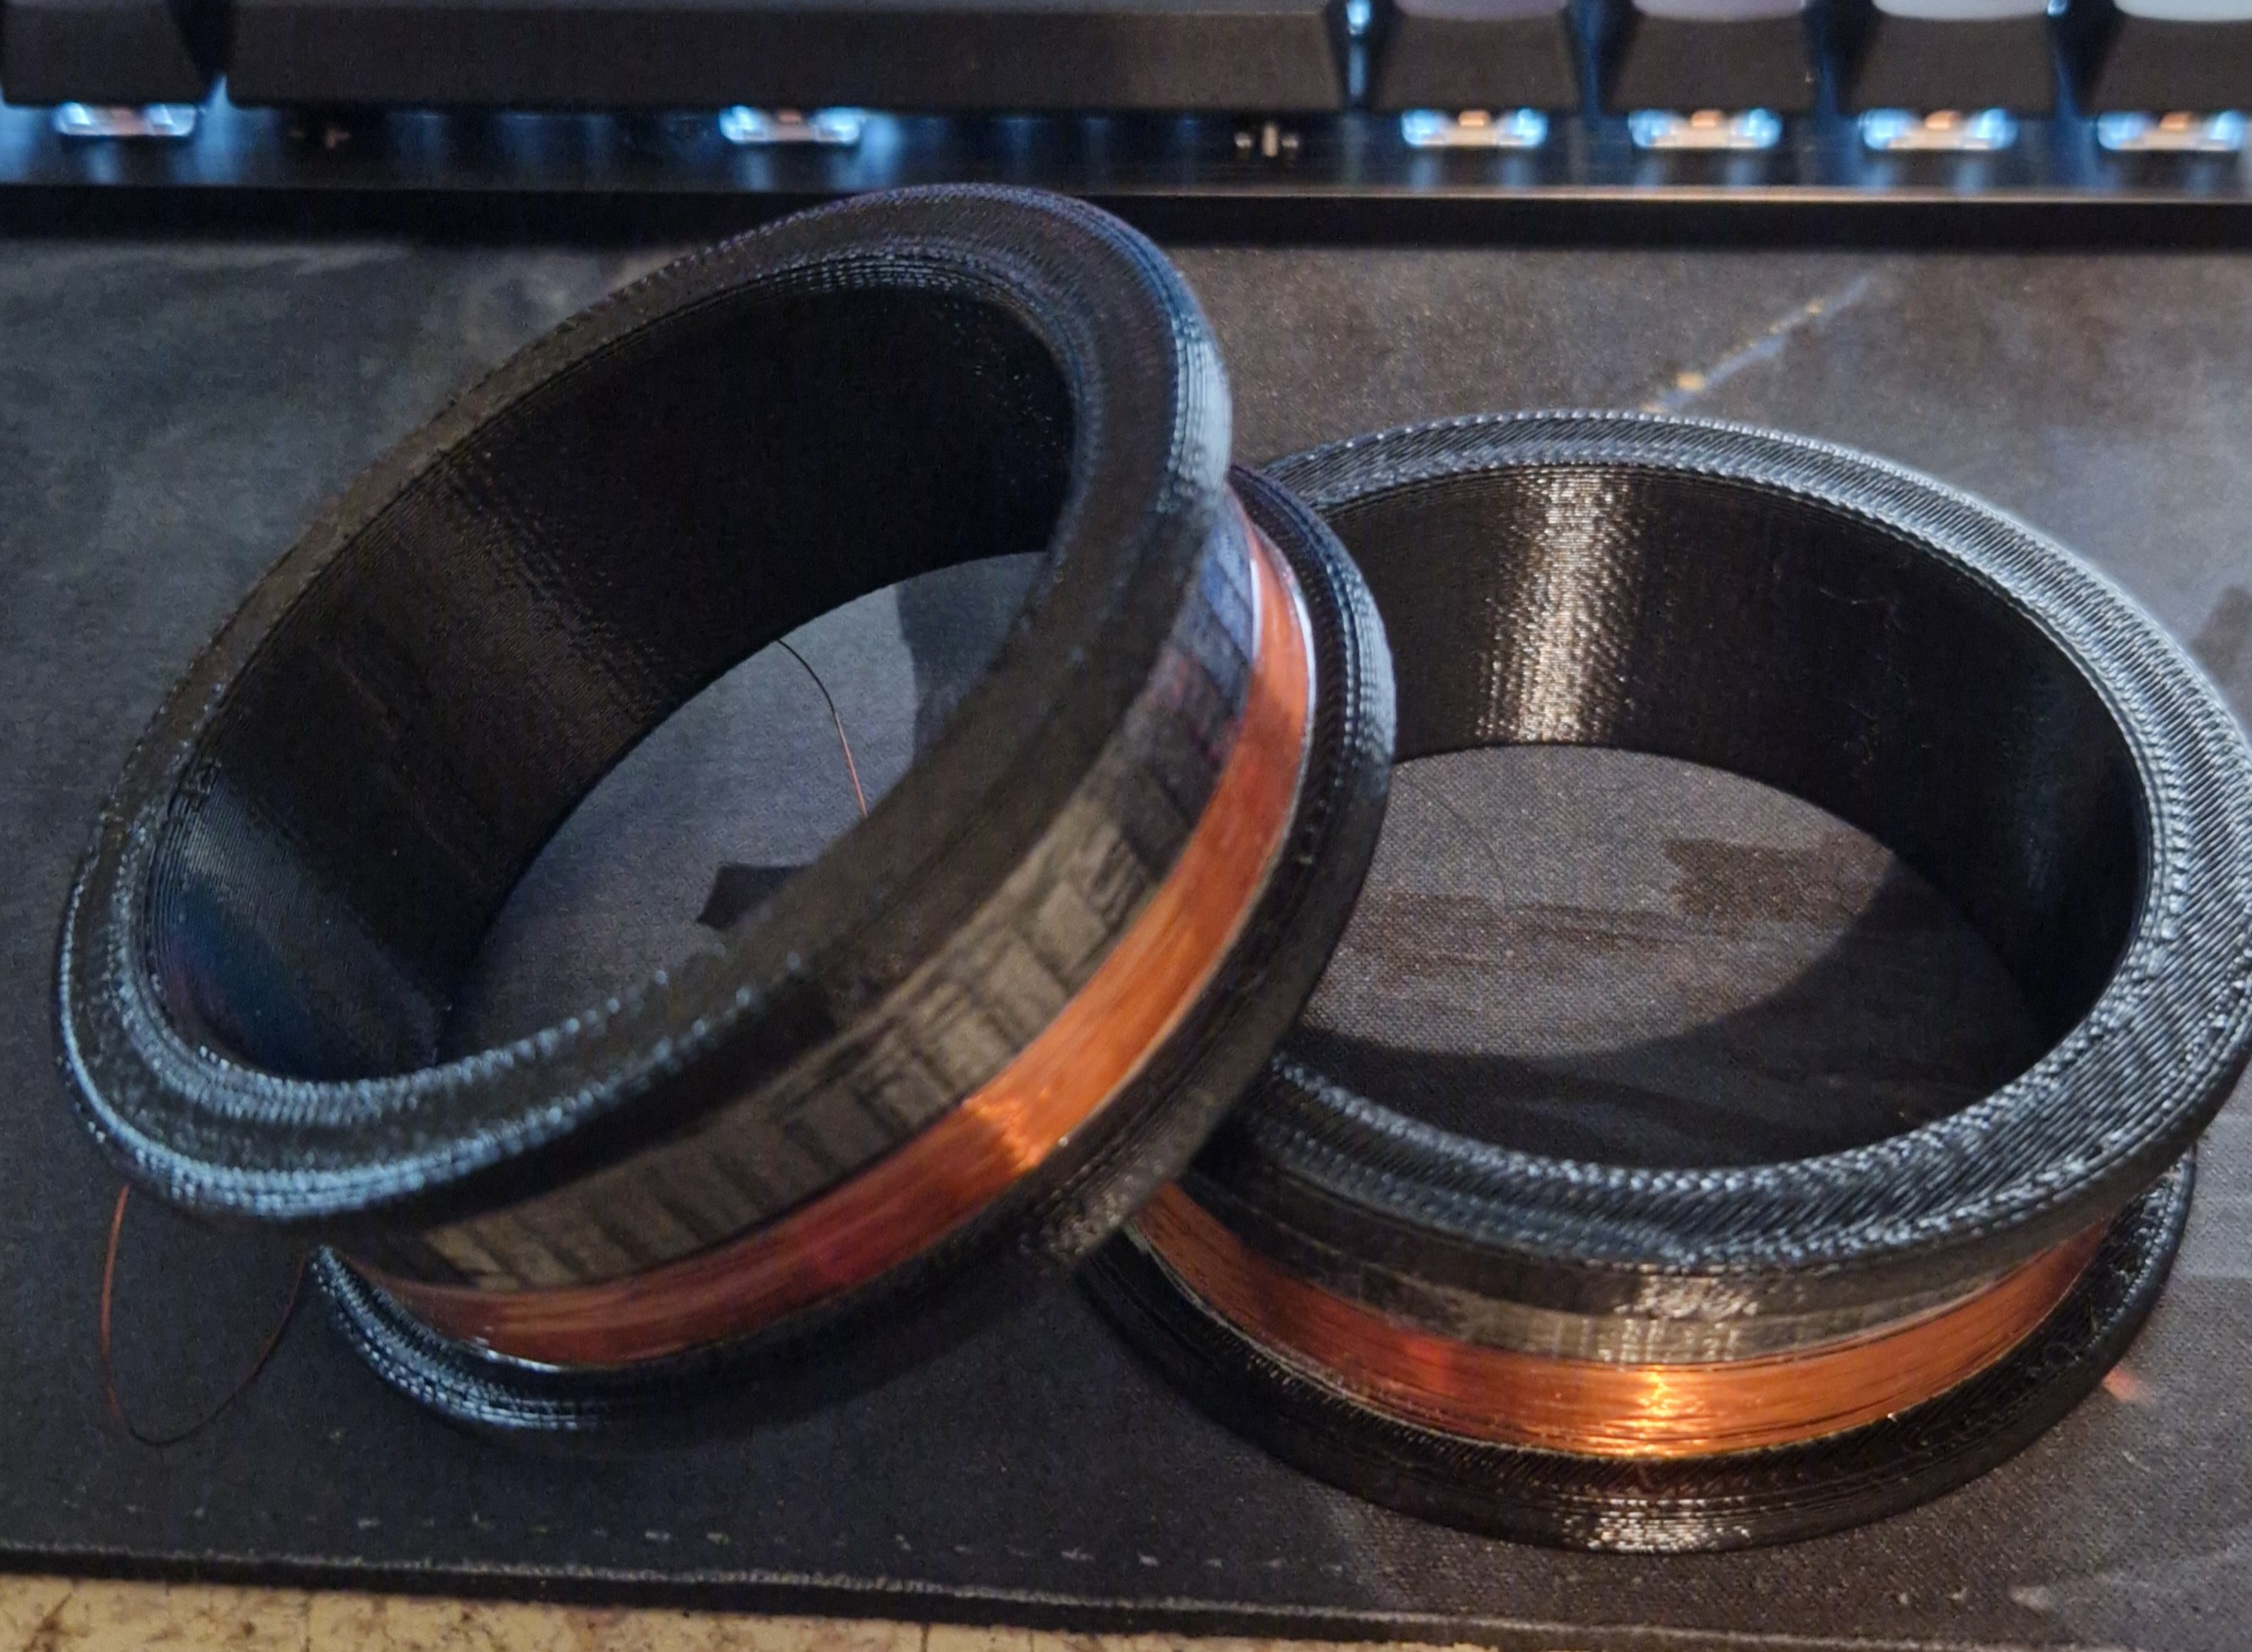
\includegraphics[width=0.4\textwidth]{assets/3d-printed-coil.jpg}
    \caption{3D Printed Coils}
    \label{fig:helmholtz-coil-3d-printed}
\end{figure}

\newpage{}
\thispagestyle{plain}

Also created a board to connect the coils to the circuit easliy. In next steps, we'll use more than one resistor and inductor, so we have designed the board to connect them easily.

\begin{figure}[h]
    \centering
    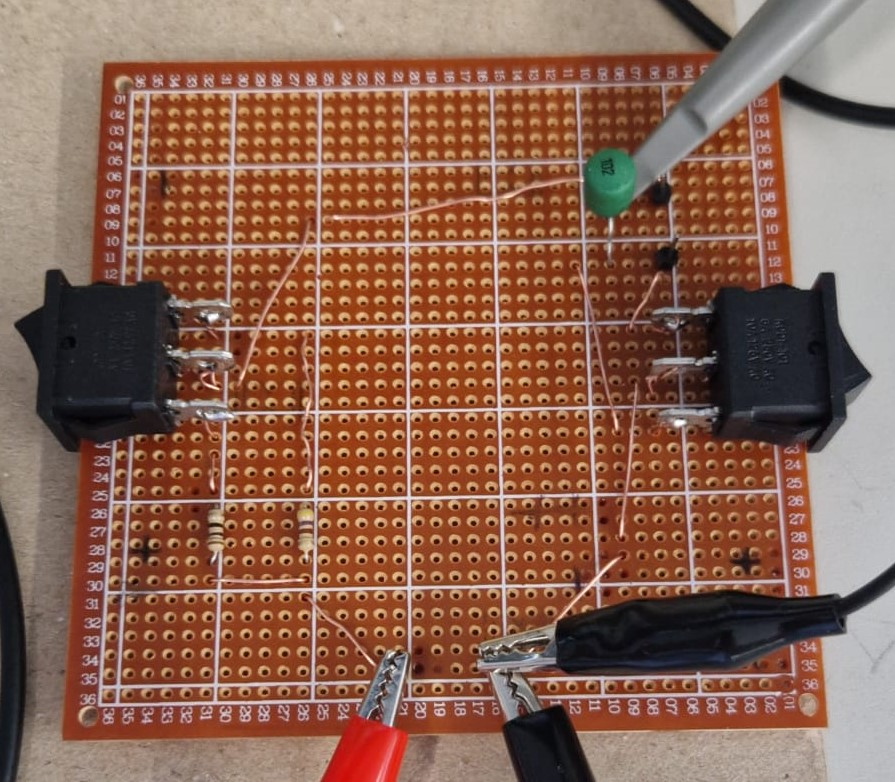
\includegraphics[width=0.3\textwidth]{assets/prototype-board.jpg}
    \caption{Prototype Board}
    \label{fig:prototype-board}
\end{figure}

\section{Measurement System}

We set up a simple RL circuit using our 3D printed coils. Used a $470\Omega (466\Omega)$ resistor and a sinusodial wave generator at $4V_{pp}(4.16V_{pp})$ $1kHz$ frequency.   

% draw the circuit diagram
\begin{figure}[h]
    \centering
    \begin{circuitikz}
        \draw (0,0) to[sinusoidal voltage source, l=$V_{in}$] (0,4)
        to[R, l=$R$] (4,4)
        to[L, l=$L$] (4,0)
        to[short] (0,0);
    \end{circuitikz}
    \caption{RL Circuit}
    \label{fig:rl-circuit}
\end{figure}

And divided input and output voltages. To find the inductance of the coil, we made circuit analysis in phasor domain and used the following formula:

\begin{align*}
    v_{out} &= L \cdot \frac{\partial i}{\partial t} \Rightarrow V_{out}(\omega) = Lj\omega I \\
    I &= \frac{V_{in}}{R + j\omega L} \\
    V_{out} &= Lj\omega \cdot \frac{V_{in}}{R + j\omega L} \\
    \frac{V_{out}}{V_{in}} &= \frac{Lj\omega}{R + j\omega L} \Rightarrow \frac{|V_{out}|}{|V_{in}|} = \frac{\omega L}{\sqrt{R^2 + \omega^2L^2}} \\
    &\boxed{\frac{|V_{out}|}{|V_{in}|} = \frac{2\pi f L}{\sqrt{R^2 + (2\pi f L)^2}}} \\
\end{align*}

\newpage{}
\thispagestyle{plain}

\subsection{System Validation}
To validate the system, we used a $1mH$ inductor and measured the output voltage. Signal generator set to $1kHz$ frequency and $4V_{pp}$ amplitude. Even thoug we set the input voltage to $4V_{pp}$, we red $4.16V_{pp}$ on the oscilloscope: 

\begin{figure}[h]
    \centering
    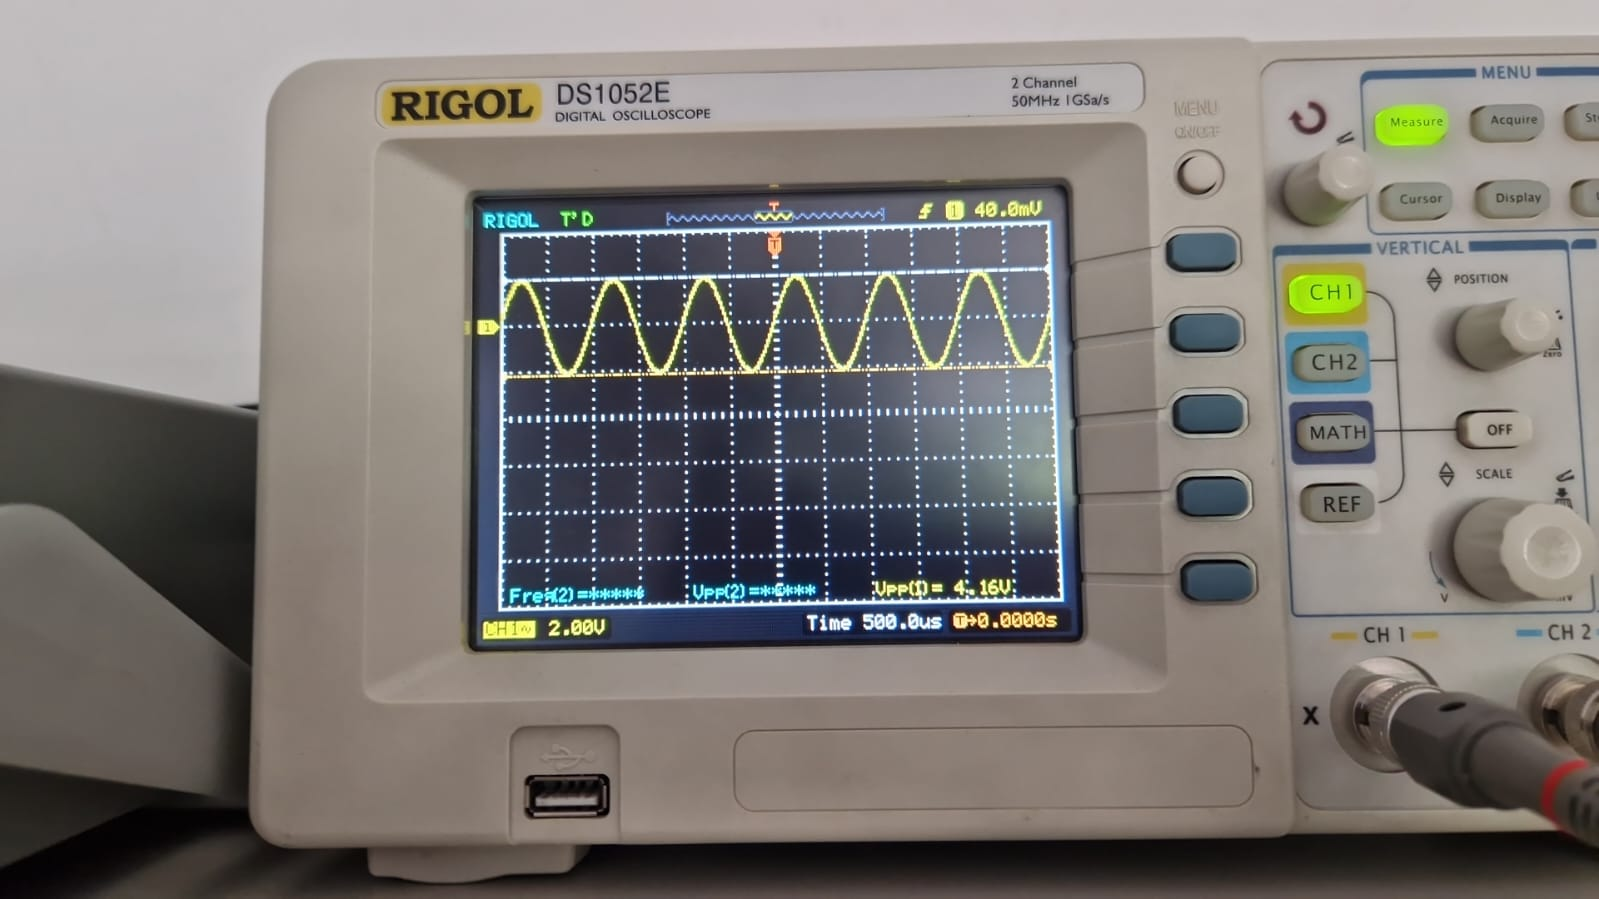
\includegraphics[width=0.9\textwidth]{assets/1k-input.jpg}
    \caption{$4V_{pp}$ Signal Generator Output}
    \label{fig:1k-signal-generator-output}
\end{figure}

And connected the $1mH$ inductor to the circuit and measured the output voltage:

\begin{figure}[h]
    \centering
    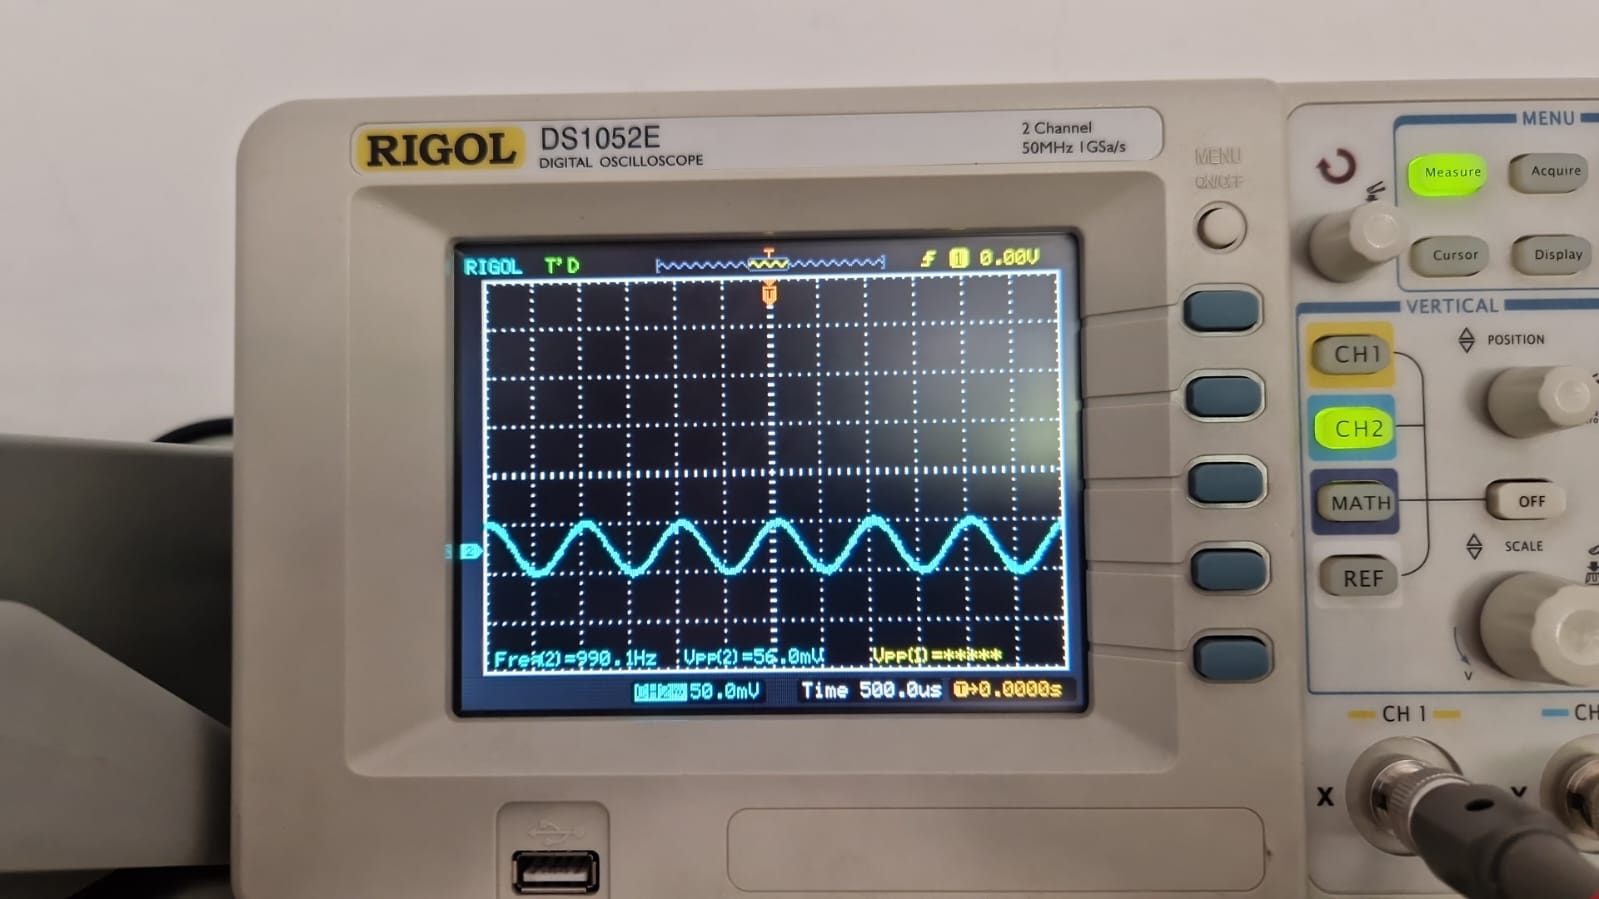
\includegraphics[width=0.9\textwidth]{assets/1k-1m-output.jpeg}
    \caption{1mH Inductor Output}
    \label{fig:1k-1m-output}
\end{figure}

\newpage{}
\thispagestyle{plain}

After putting every value to the formula, we found the inductance of the coil as follows:

\begin{align*}
    \frac{|V_{out}|}{|V_{in}|} &= \frac{2\pi f L}{\sqrt{R^2 + (2\pi f L)^2}} \\
    \Rightarrow \frac{27 \cdot 10^{-3}}{213 \cdot 10^{-2}} &= \frac{2\pi \cdot 10^3 \cdot L}{\sqrt{466^2 + (2\pi \cdot 10^3 \cdot L)^2}} \\
    L &\approx 0.00094H \approx 0.94mH
\end{align*}

It is very close to the actual value of the inductor, so we can say that our system and theoretical calculation is working properly.

\section{Calculating the Inductance of the Helmholtz Coil}

\subsection{Theoretical Calculation}

The inductance of a Helmholtz coil can be calculated using the following formula:

\[ L = \frac{\mu N^2A}{l} \]

\noindent Where:
\begin{itemize}
    \item \( \mu \) is the permeability of the air ($4\pi \cdot 10^{-7}H/m$, \cite{air_permeability_saini})
    \item \( N \) is the number of windings
    \item \( A \) is the area of the coil
    \item \( l \) is the length of the coil
\end{itemize}

According to the formula, the inductance of the Helmholtz coil is calculated as follows:

\begin{align*}
    L &= \frac{4\pi \times 10^{-7} \times 30^2 \times \pi \times 0.04^2}{0.009} \\
    &\approx 0.00063H \approx 0.63mH~\text{For one coil} \\
    &\approx 0.00126H \approx 1.26mH~\text{For two coils}
\end{align*}

\newpage{}
\thispagestyle{plain}

\subsection{Experimental Calculation}

The theoretical inductance of Helmholtz Coil is \( 1.26mH \). To find the real inductance, we changed the $1mH$ inductor from the circuit before and connected the Helmholtz coil to the circuit. Input voltage, resistor and frequency are the same as the previous experiment. Output voltage is as follows:

\begin{figure}[h]
    \centering
    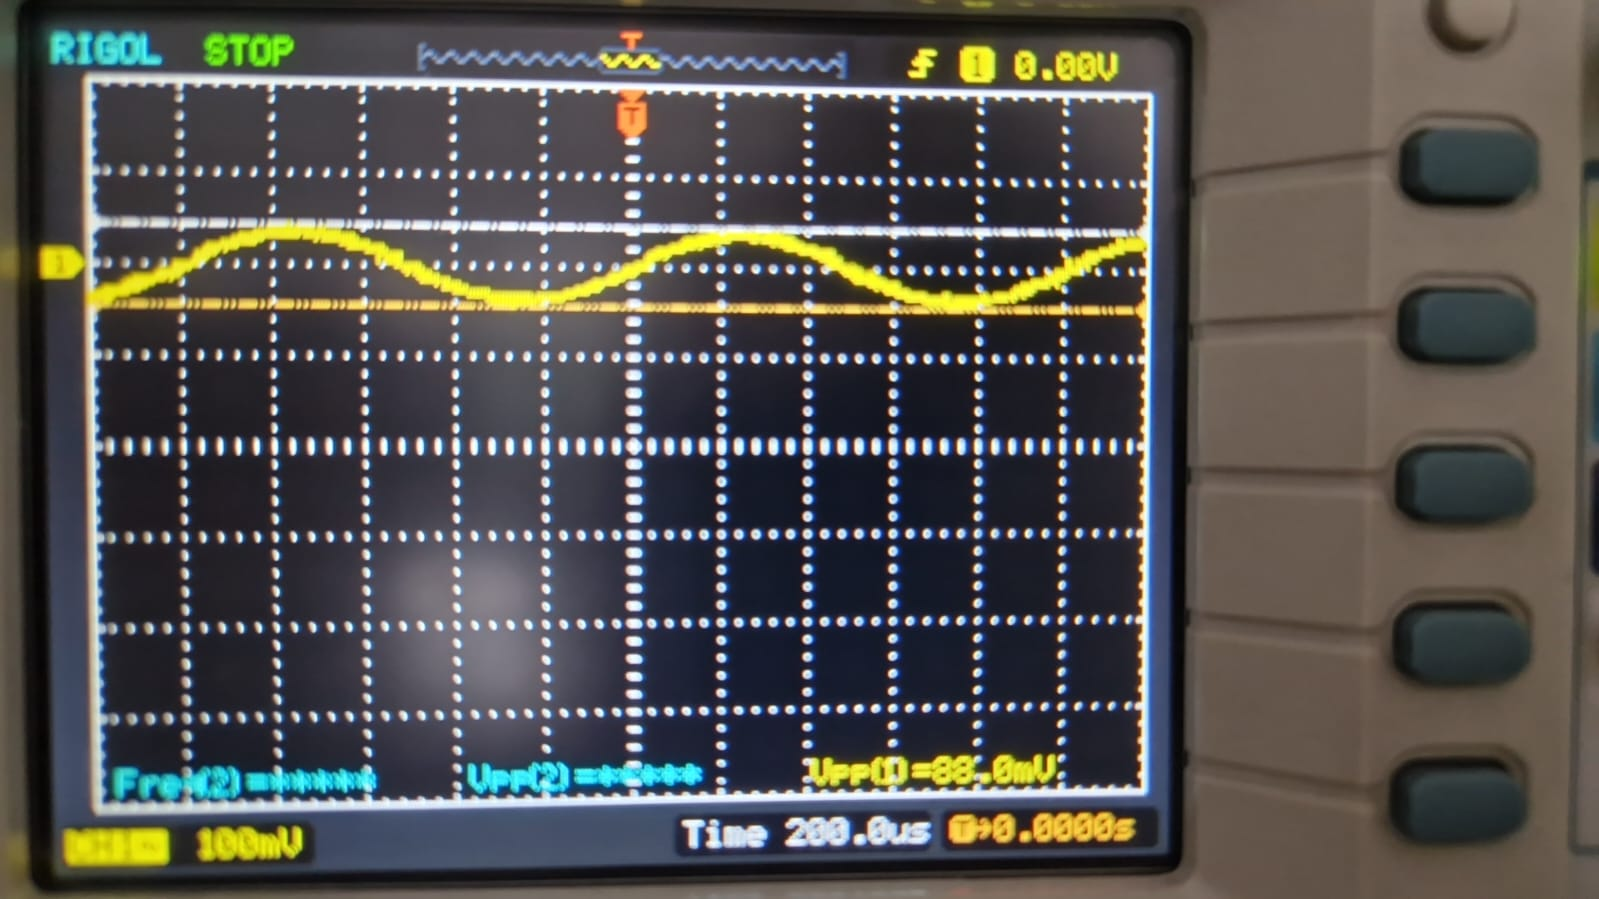
\includegraphics[width=0.9\textwidth]{assets/1k-helmholtz-output.jpg}
    \caption{Helmholtz Coil Output}
    \label{fig:1k-helmholtz-output}
\end{figure}

Output reads $88mV_{pp}$ on the oscilloscope. After putting every value to the formula, we found the inductance of the coil as follows:

\begin{align*}
    \frac{|V_{out}|}{|V_{in}|} &= \frac{2\pi f L}{\sqrt{R^2 + (2\pi f L)^2}} \\
    \Rightarrow \frac{44 \cdot 10^{-3}}{213 \cdot 10^{-2}} &= \frac{2\pi \cdot 10^3 \cdot L}{\sqrt{466^2 + (2\pi \cdot 10^3 \cdot L)^2}} \\
    L &\approx 0.00153H \approx 1.53mH
\end{align*}

Real inductance is \( 1.53mH \) which is very close to the theoretical value $1.26mH$. We can say that our system is working properly. Difference between the theoretical and experimental values can be due to the imperfections in the coil design and different magnetic properties of the materials used in the coil.

Now we are about to analyze the frequency response of the RL circuit with the Helmholtz coil with the following frequencies:

\begin{align*}
    f &= 1/T \\
    T &= 10L/R = 0.0015s \implies f = 666Hz \\
    T &= L/R = 0.00015s \implies f = 6.66kHz \\
    T &= L/10R = 0.000015s \implies f = 66.66kHz
\end{align*}

\newpage{}
\thispagestyle{plain}

\subsection{Frequency Analysis}

\subsubsection{T=10L/R $\implies$ f=666Hz}

\begin{figure}[h]
    \centering
    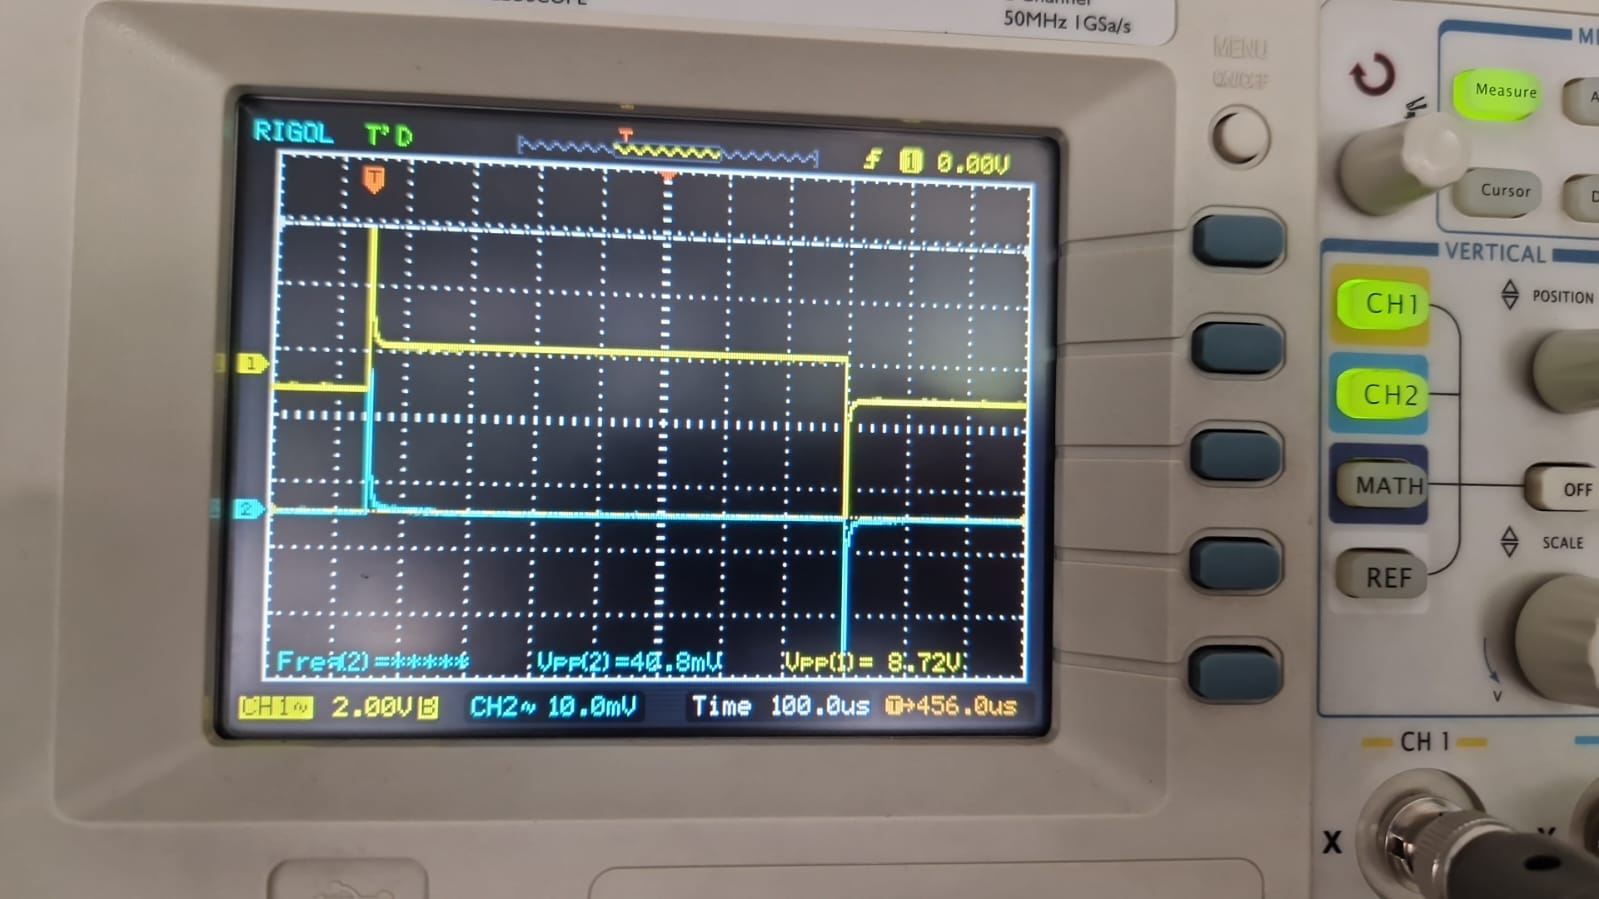
\includegraphics[width=0.9\textwidth]{assets/666-hz-5vpp.jpg}
    \caption{666Hz Output @ $5V_{pp}$}
    \label{fig:666-hz-5vpp-output}
\end{figure}

\begin{figure}[h]
    \centering
    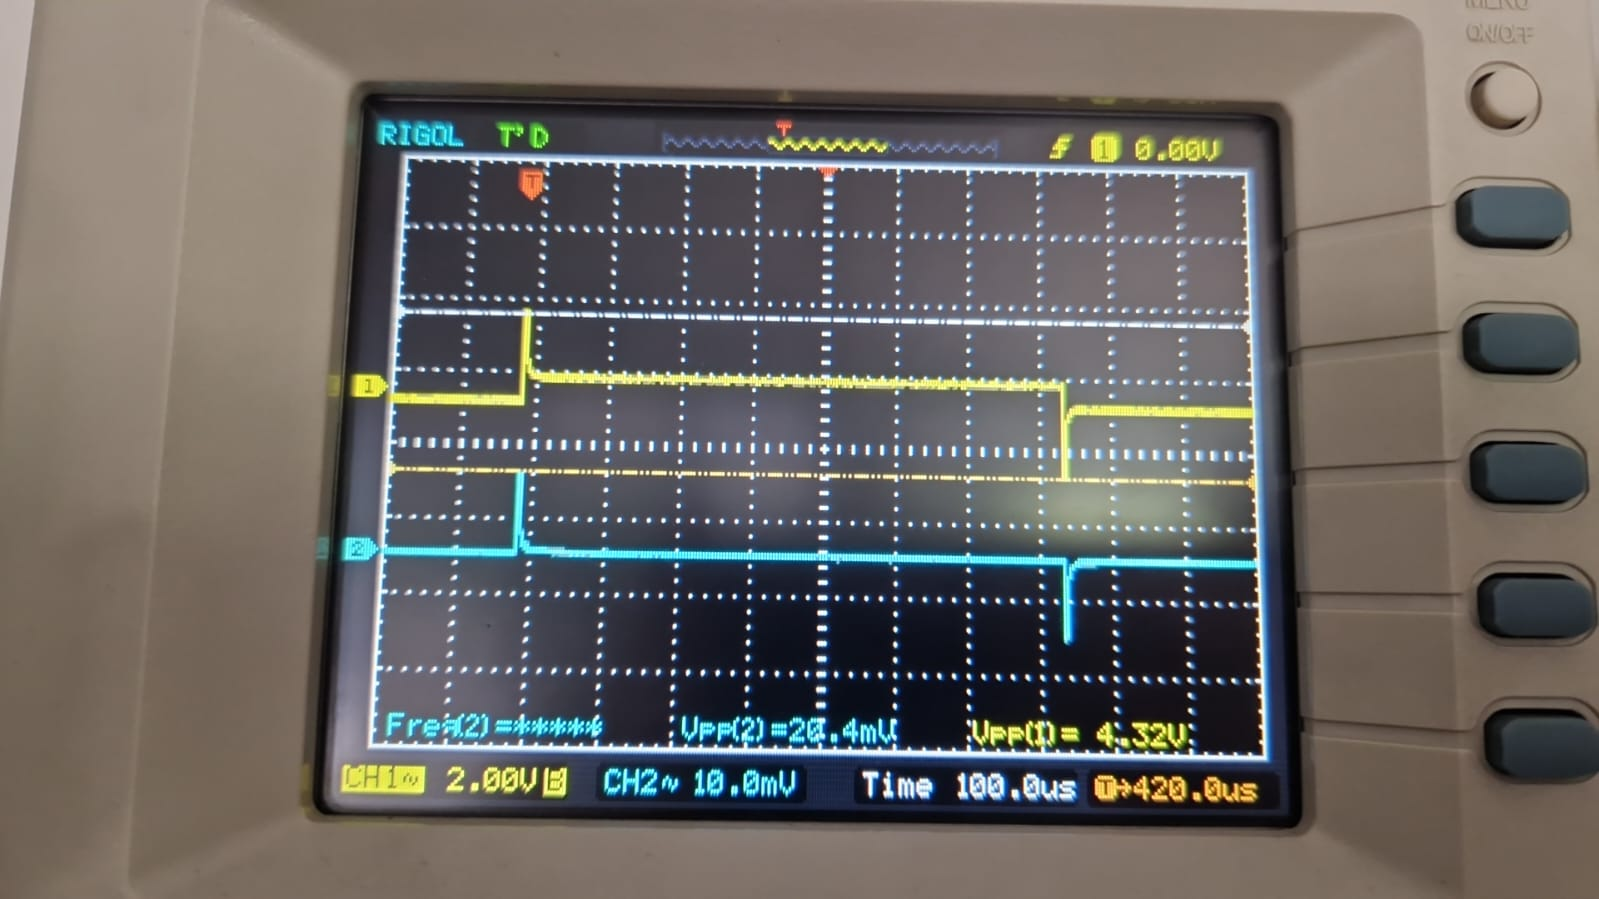
\includegraphics[width=0.9\textwidth]{assets/666-hz-2.5vpp.jpg}
    \caption{666Hz Output @ $2.5V_{pp}$}
    \label{fig:666-hz-2.5vpp-output}
\end{figure}

\begin{itemize}
    \item The period is long enough for the inductor to fully charge and discharge within each half-cycle.
    \item The voltage across the inductor shows a complete exponential rise and fall.
\end{itemize}

\newpage{}
\thispagestyle{plain}

\subsubsection{T=L/R $\implies$ f=6.66kHz}

\begin{figure}[h]
    \centering
    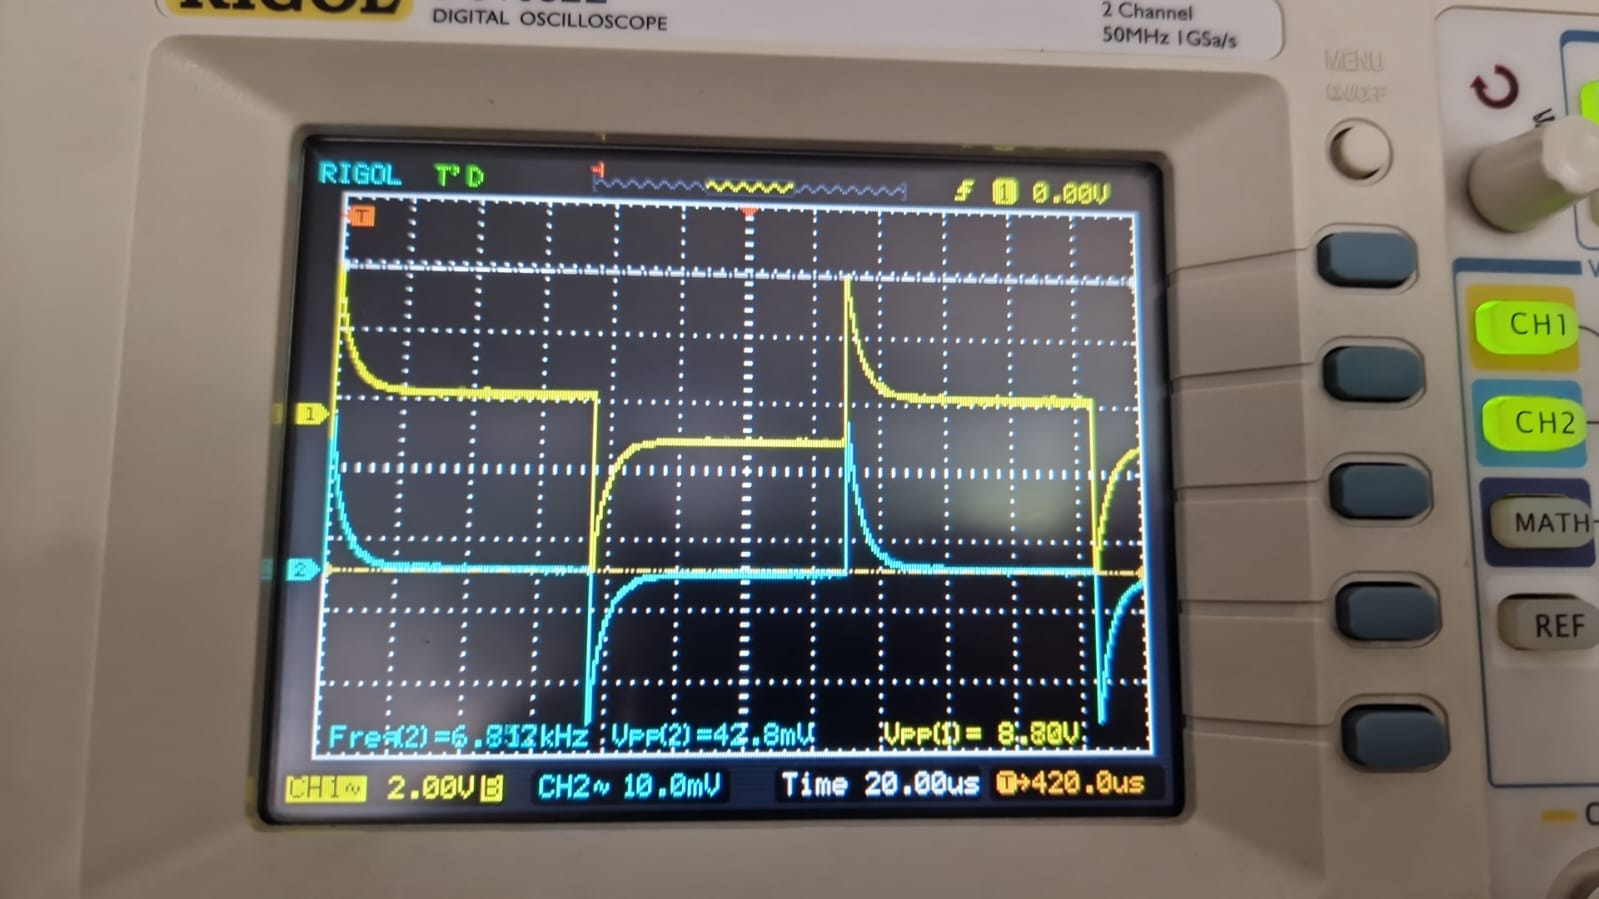
\includegraphics[width=0.9\textwidth]{assets/6666-hz-5vpp.jpg}
    \caption{6.66kHz Output @ $5V_{pp}$}
    \label{fig:6666-hz-5vpp-output}
\end{figure}

\begin{figure}[h]
    \centering
    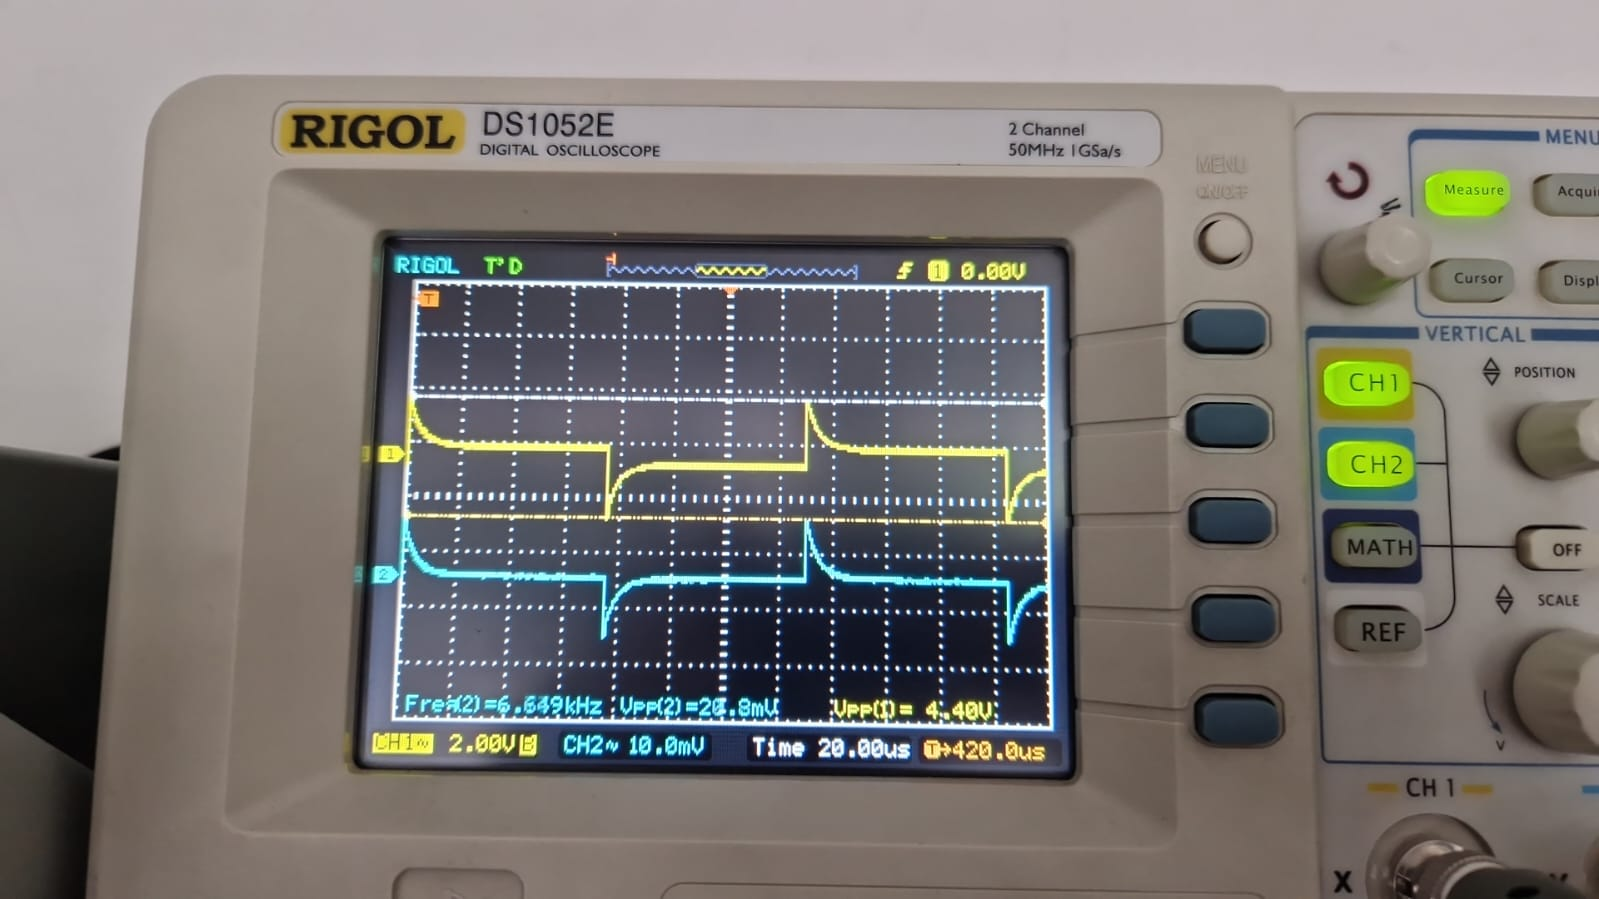
\includegraphics[width=0.9\textwidth]{assets/6666-hz-2.5vpp.jpg}
    \caption{6.66kHz Output @ $2.5V_{pp}$}
    \label{fig:6666-hz-2.5vpp-output}
\end{figure}

\begin{itemize}
    \item The period is equal to the time constant, allowing partial charging and discharging.
    \item The voltage across the inductor shows partial exponential rise and fall.
\end{itemize}

\newpage{}
\thispagestyle{plain}

\subsubsection{T=L/10R $\implies$ f=66.66kHz}

\begin{figure}[h]
    \centering
    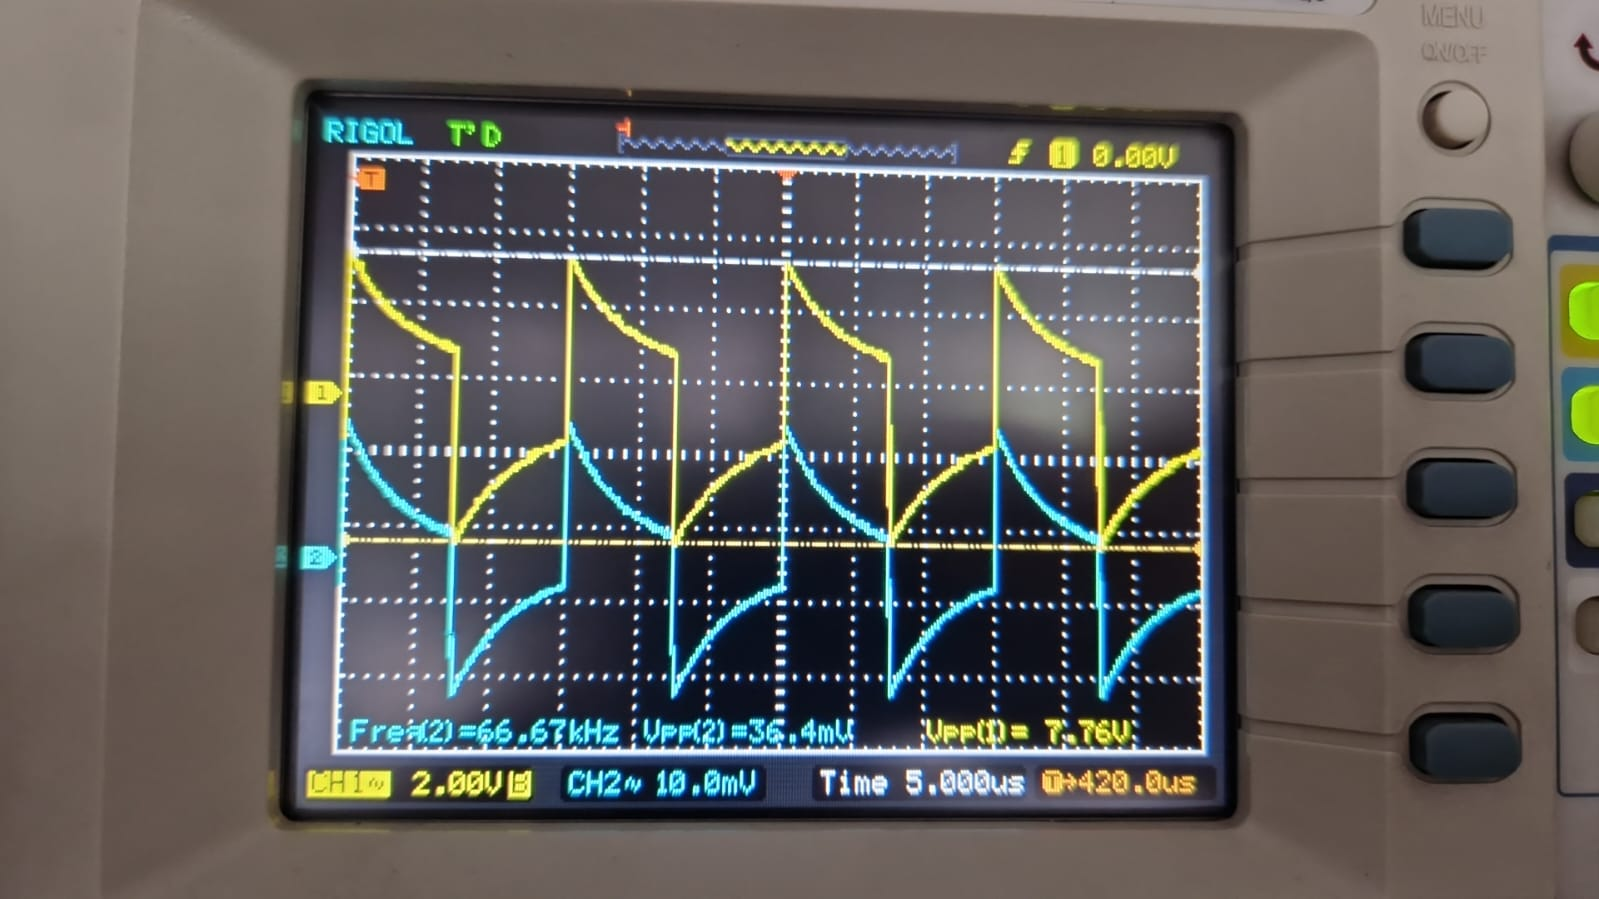
\includegraphics[width=0.9\textwidth]{assets/66666-hz-5vpp.jpg}
    \caption{66.66kHz Output @ $5V_{pp}$}
    \label{fig:66666-hz-5vpp-output}
\end{figure}

\begin{figure}[h]
    \centering
    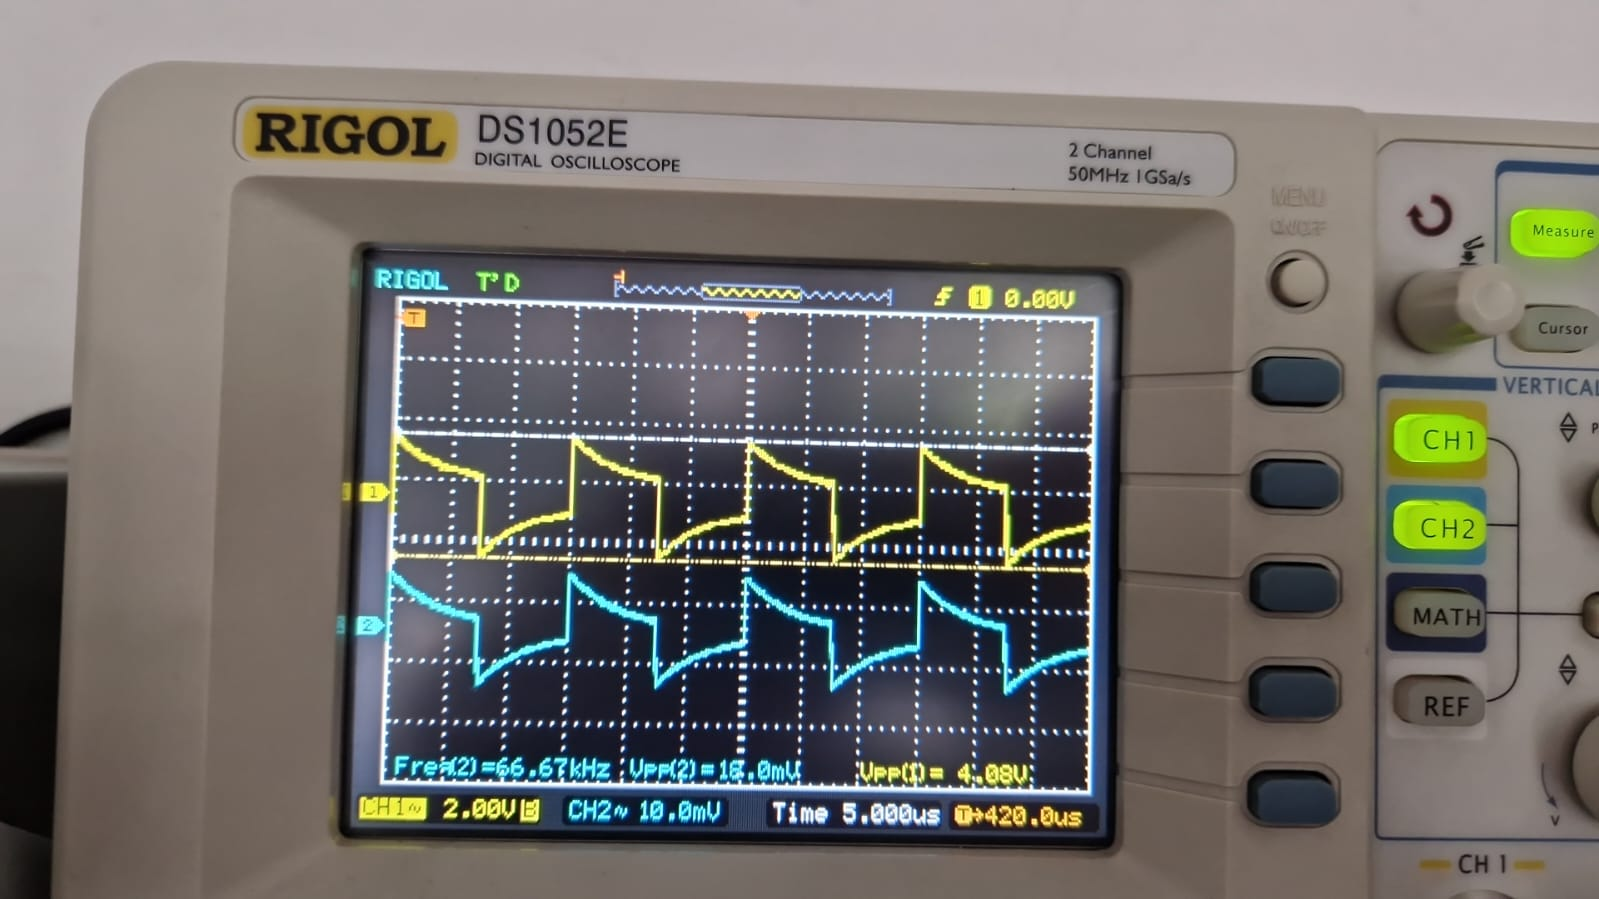
\includegraphics[width=0.9\textwidth]{assets/66666-hz-2.5vpp.jpg}
    \caption{66.66kHz Output @ $2.5V_{pp}$}
    \label{fig:66666-hz-2.5vpp-output}
\end{figure}

\begin{itemize}
    \item The period is very short, leading to minimal charging and discharging of the inductor.
    \item The voltage across the inductor barely shows any change.
\end{itemize}

\newpage{}
\thispagestyle{plain}

\subsubsection{Reducing the Amplitude}
When the amplitude of the square wave is reduced to half (0-2.5V), the voltages across both the inductor and the resistor also reduce proportionally. The overall behavior and response times remain consistent, but the magnitude of the voltages is halved.

	\chapter{Simulation in LTspice}

\section{Modeling the Helmholtz Coil}


\begin{figure}[h]
    \centering
    \begin{circuitikz} \draw
        (0,0) to[square voltage source, l=0-5V] (0,4)
        to[R, l=$10\Omega$] (4,4) 
        to[L, l=0.76mH] (4,2) 
        to[L, l=0.76mH] (4,0) -- (0,0)
        ;
    \end{circuitikz}
    \caption{Helmholtz Coil Circuit Diagram}
\end{figure}

Designed the coil in LTspice and simulated the following netlist:

\begin{lstlisting}
    * Helmholtz Coil Simulation
    V1 N001 0 PULSE(0 5 0 {t_edge} {t_edge} {1/2/freq-t_edge} {1/freq})
    R1 VL1 N001 10
    L1 VL1 P001 0.76m
    L2 P001 0 0.76m
    .tran 0 10m 0 1u
    .param t_edge=1u freq=666
    .ic V(VL1)=0
    .backanno
    .end
\end{lstlisting}

\newpage{}
\thispagestyle{plain}

\section{Frequency Analysis}
\subsubsection{T=10L/R $\implies$ f=666Hz}

\begin{figure}[h]
    \centering
    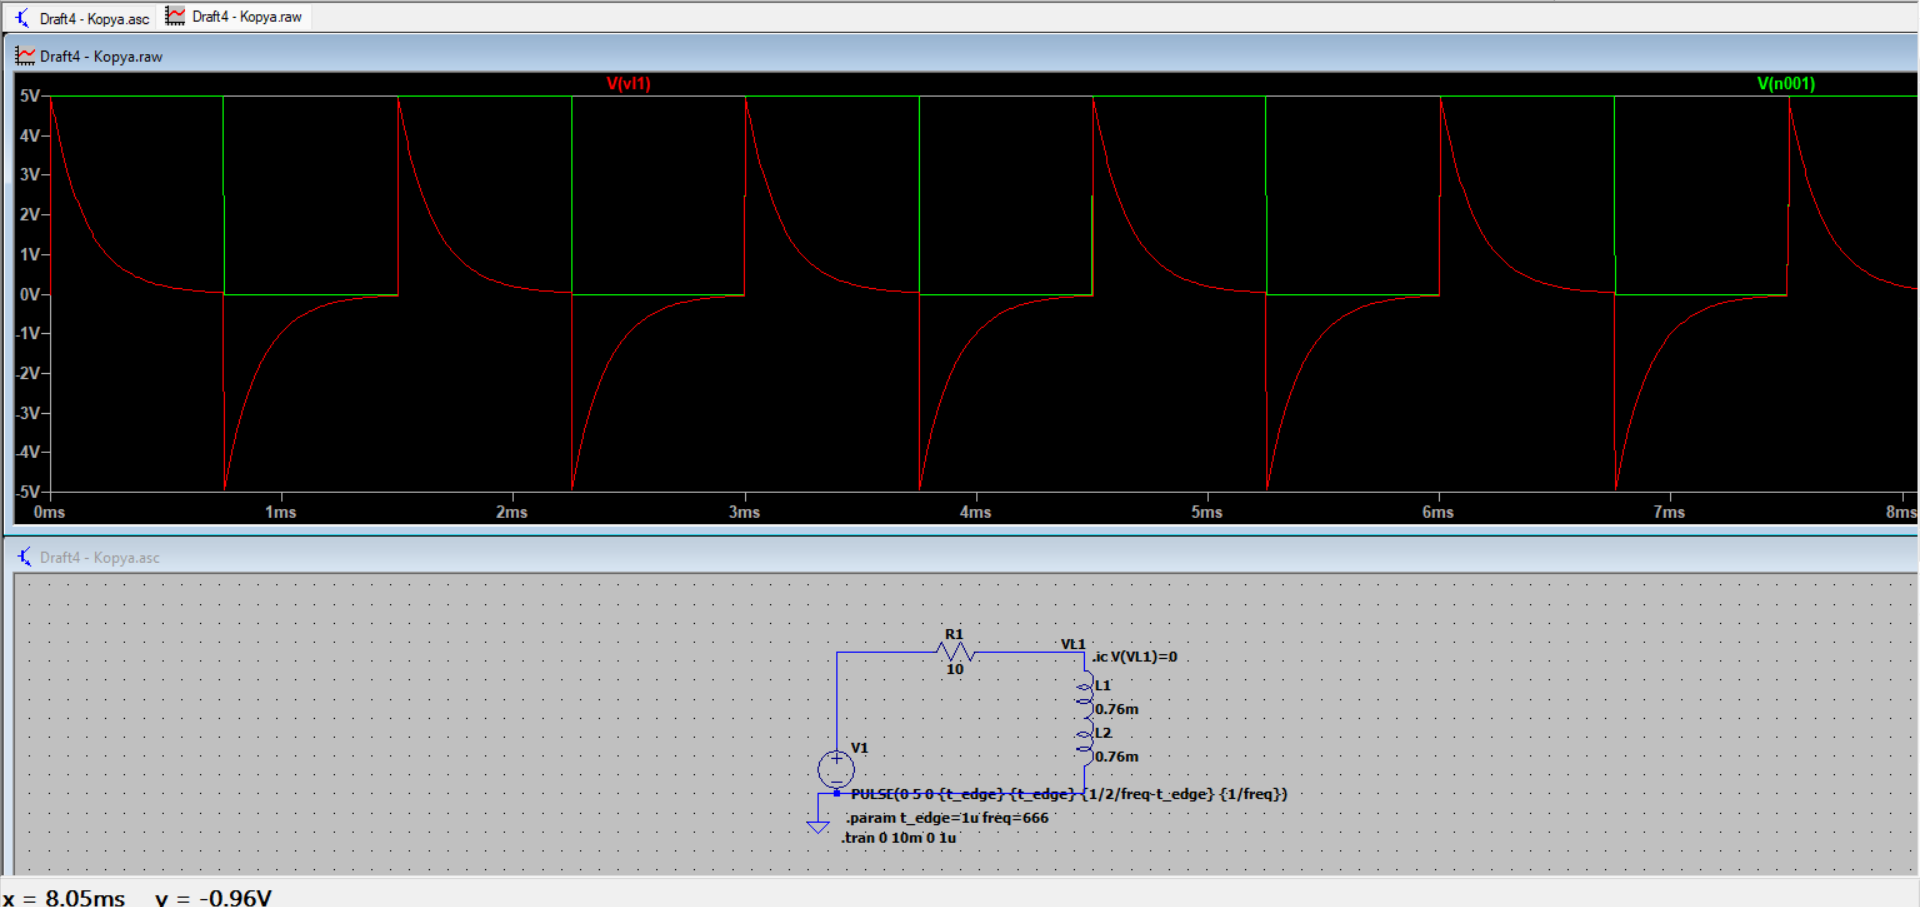
\includegraphics[width=1\textwidth]{assets/666-hz-5vpp-sim.png}
    \caption{666Hz Output @ $5V_{pp}$}
    \label{fig:666-hz-5vpp-output}
\end{figure}

\begin{figure}[h]
    \centering
    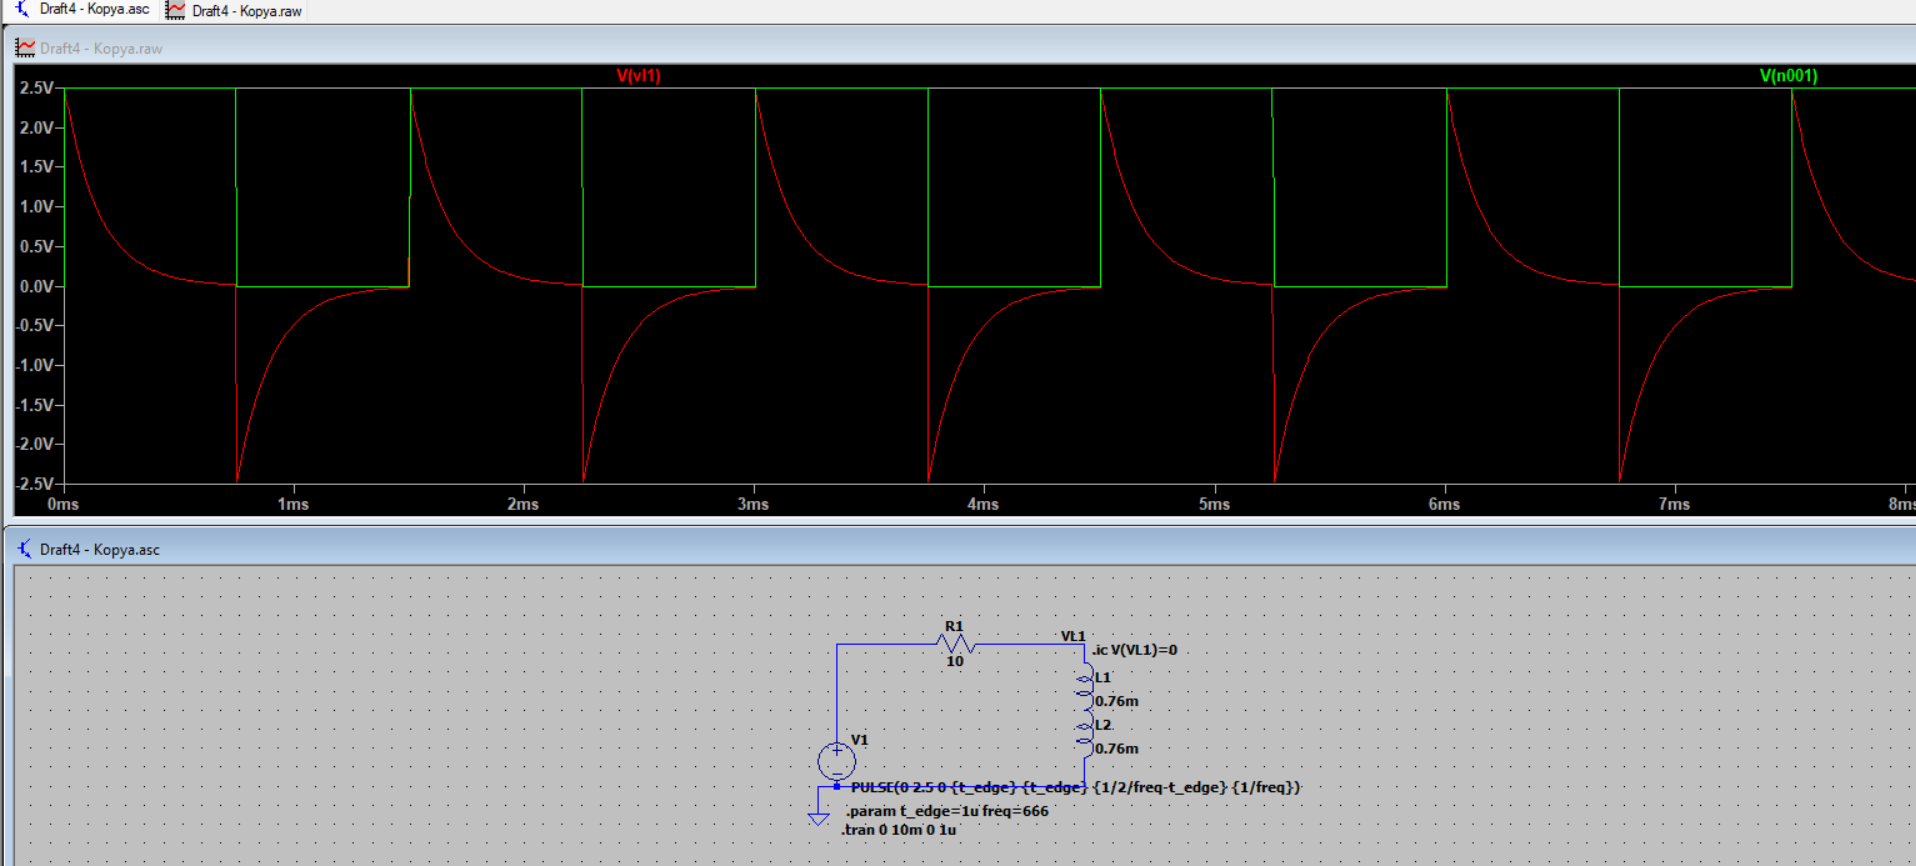
\includegraphics[width=1\textwidth]{assets/666-hz-2.5vpp-sim.png}
    \caption{666Hz Output @ $2.5V_{pp}$}
    \label{fig:666-hz-2.5vpp-output}
\end{figure}

Same characteristics as the experimental results are observed in the simulation.

\newpage{}
\thispagestyle{plain}

\subsubsection{T=L/R $\implies$ f=6.66kHz}

\begin{figure}[h]
    \centering
    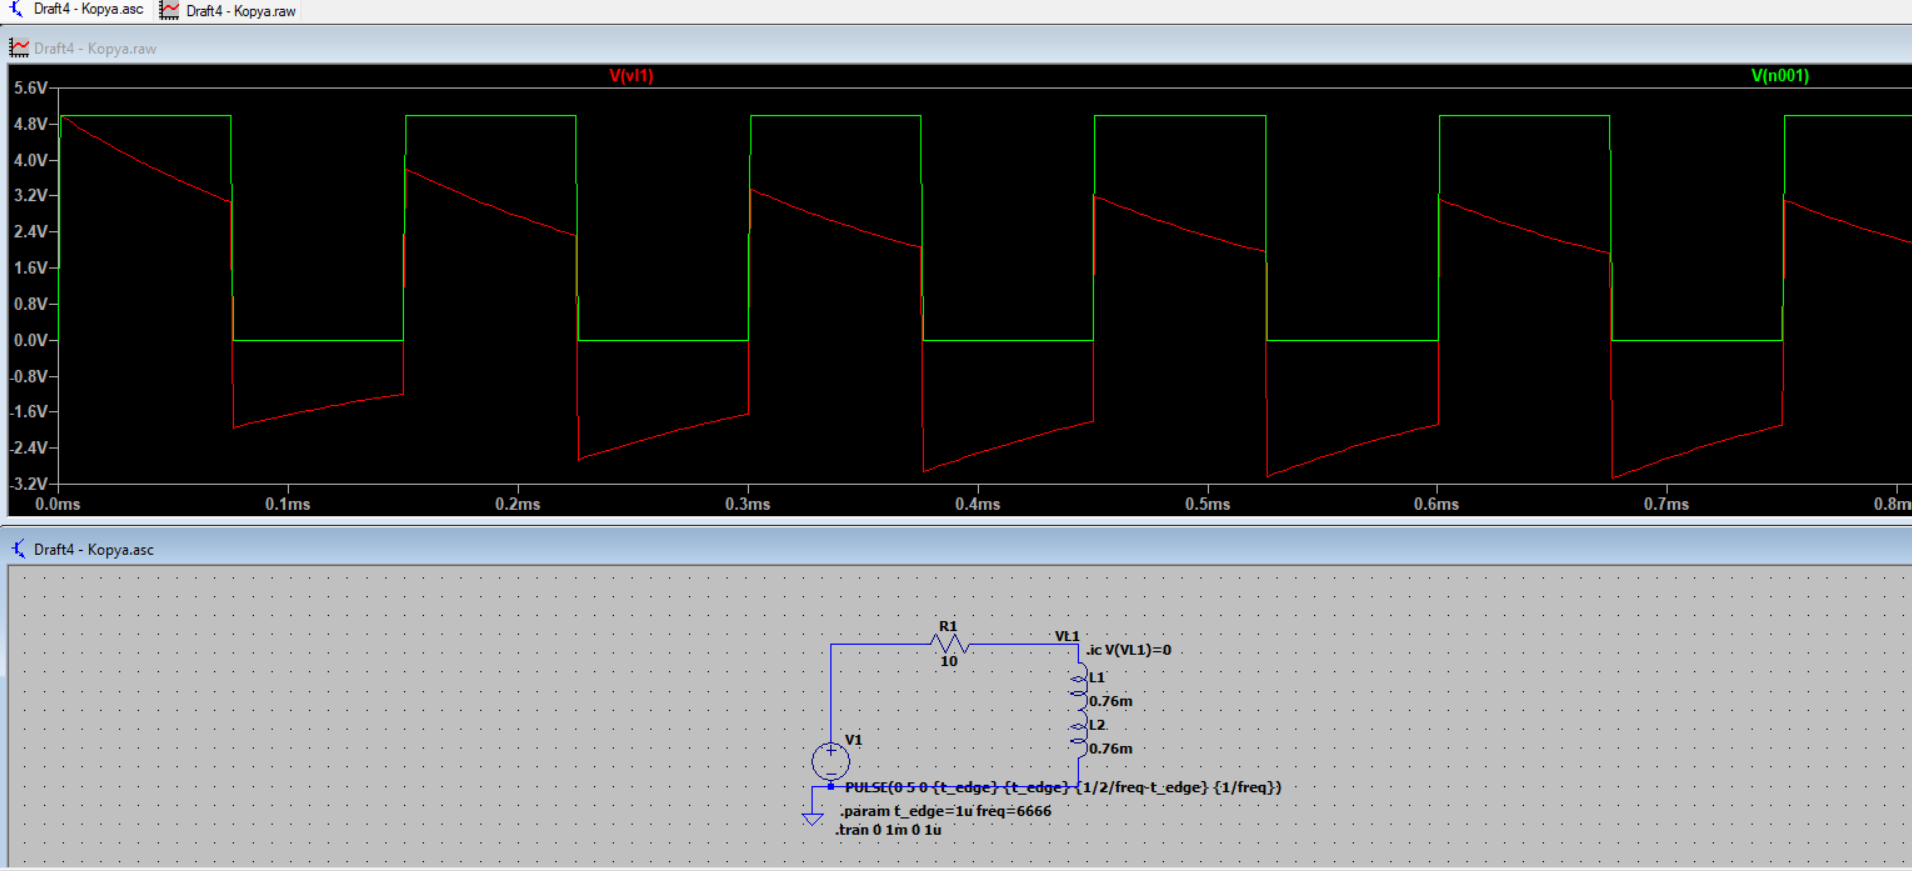
\includegraphics[width=1\textwidth]{assets/6666-hz-5vpp-sim.png}
    \caption{6.66kHz Output @ $5V_{pp}$}
    \label{fig:6666-hz-5vpp-output}
\end{figure}

\begin{figure}[h]
    \centering
    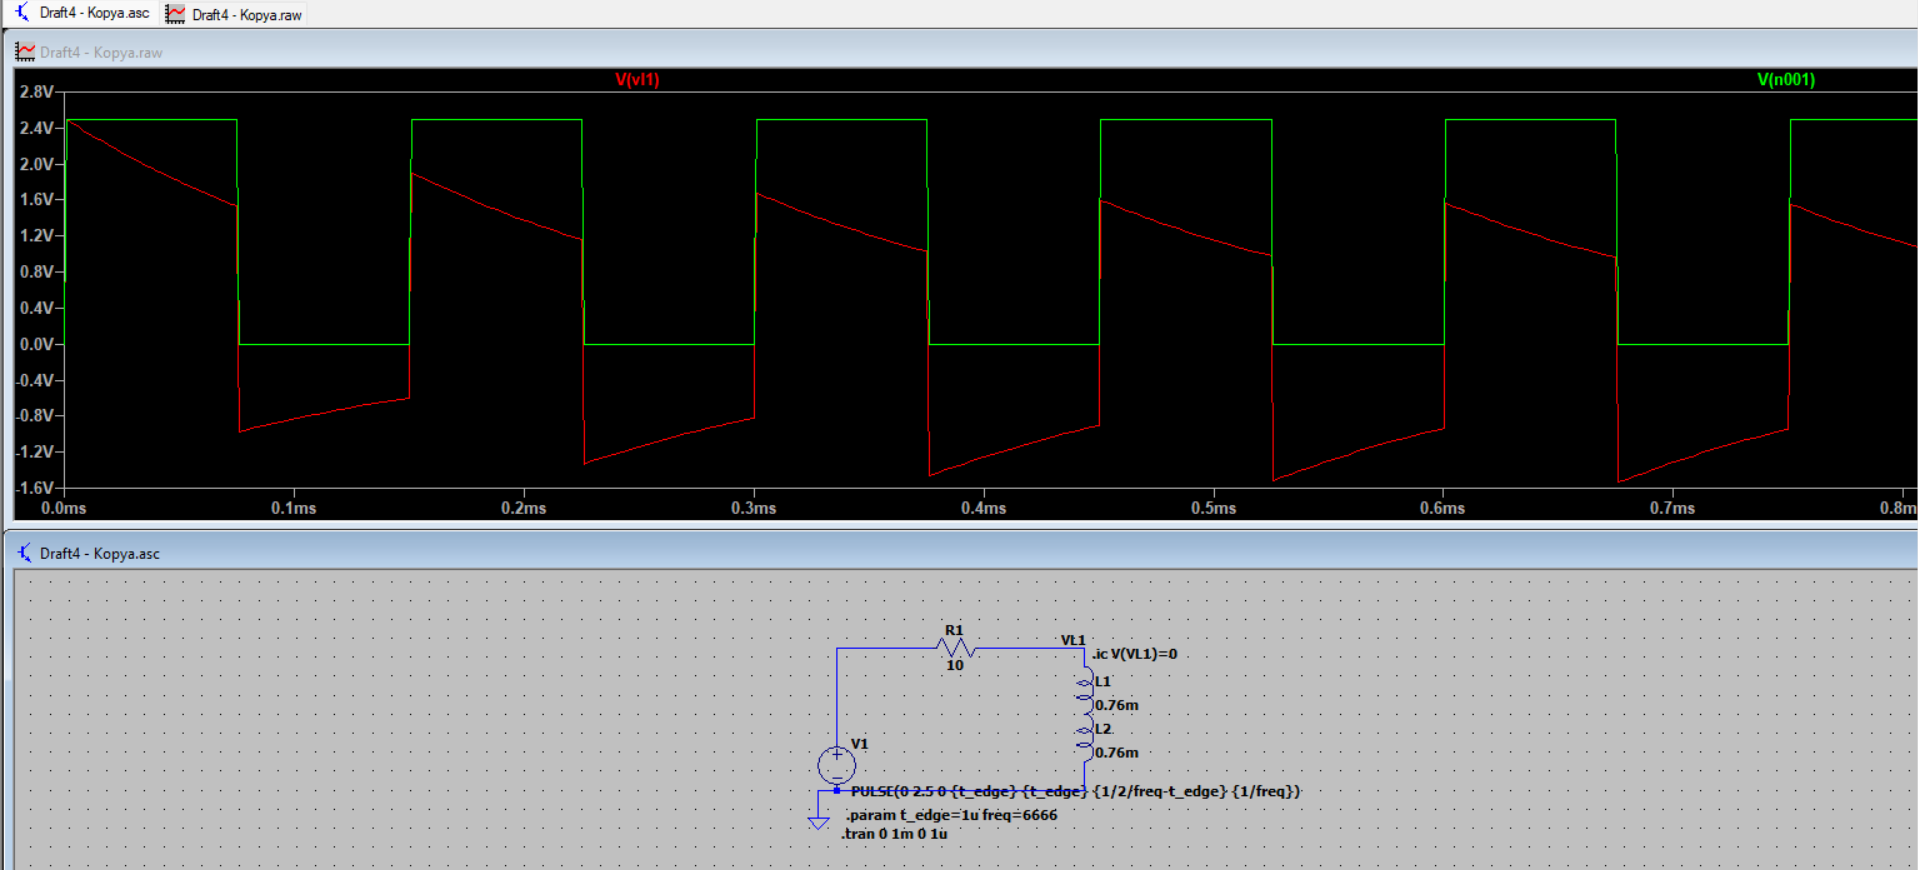
\includegraphics[width=1\textwidth]{assets/6666-hz-2.5vpp-sim.png}
    \caption{6.66kHz Output @ $2.5V_{pp}$}
    \label{fig:6666-hz-2.5vpp-output}
\end{figure}

Same characteristics as the experimental results are observed in the simulation.

\newpage{}
\thispagestyle{plain}

\subsubsection{T=L/10R $\implies$ f=66.66kHz}

\begin{figure}[h]
    \centering
    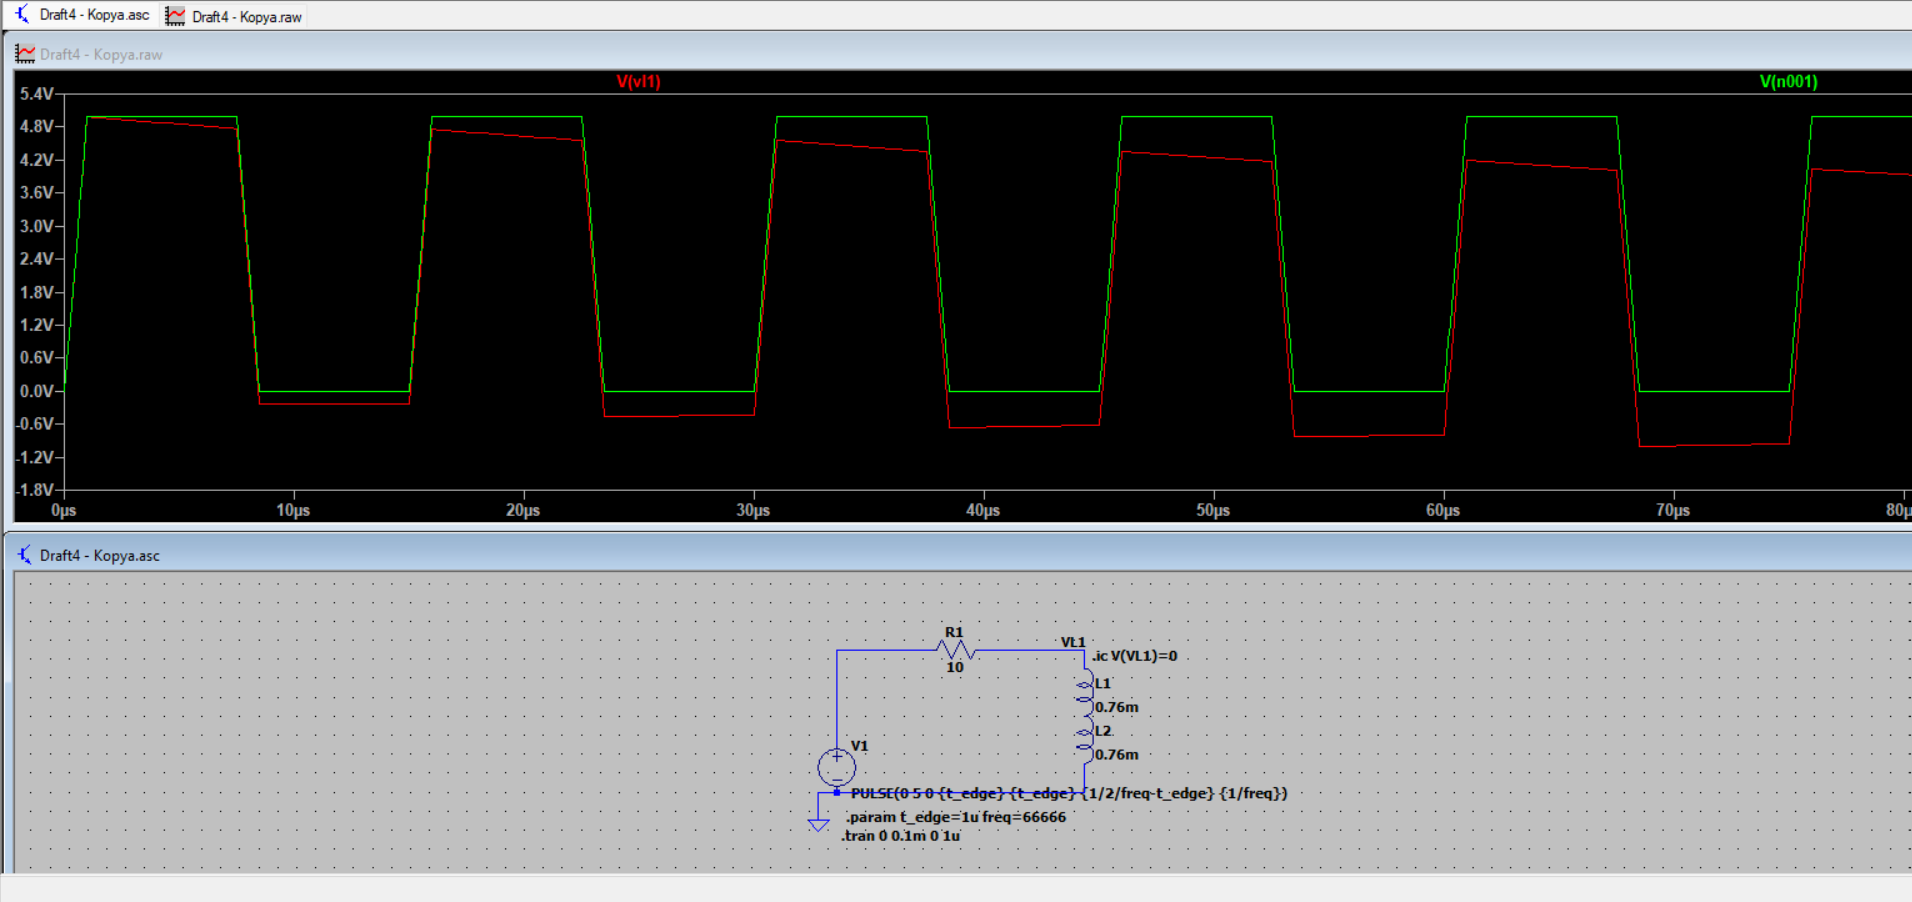
\includegraphics[width=1\textwidth]{assets/66666-hz-5vpp-sim.png}
    \caption{66.66kHz Output @ $5V_{pp}$}
    \label{fig:6666-hz-5vpp-output}
\end{figure}

\begin{figure}[h]
    \centering
    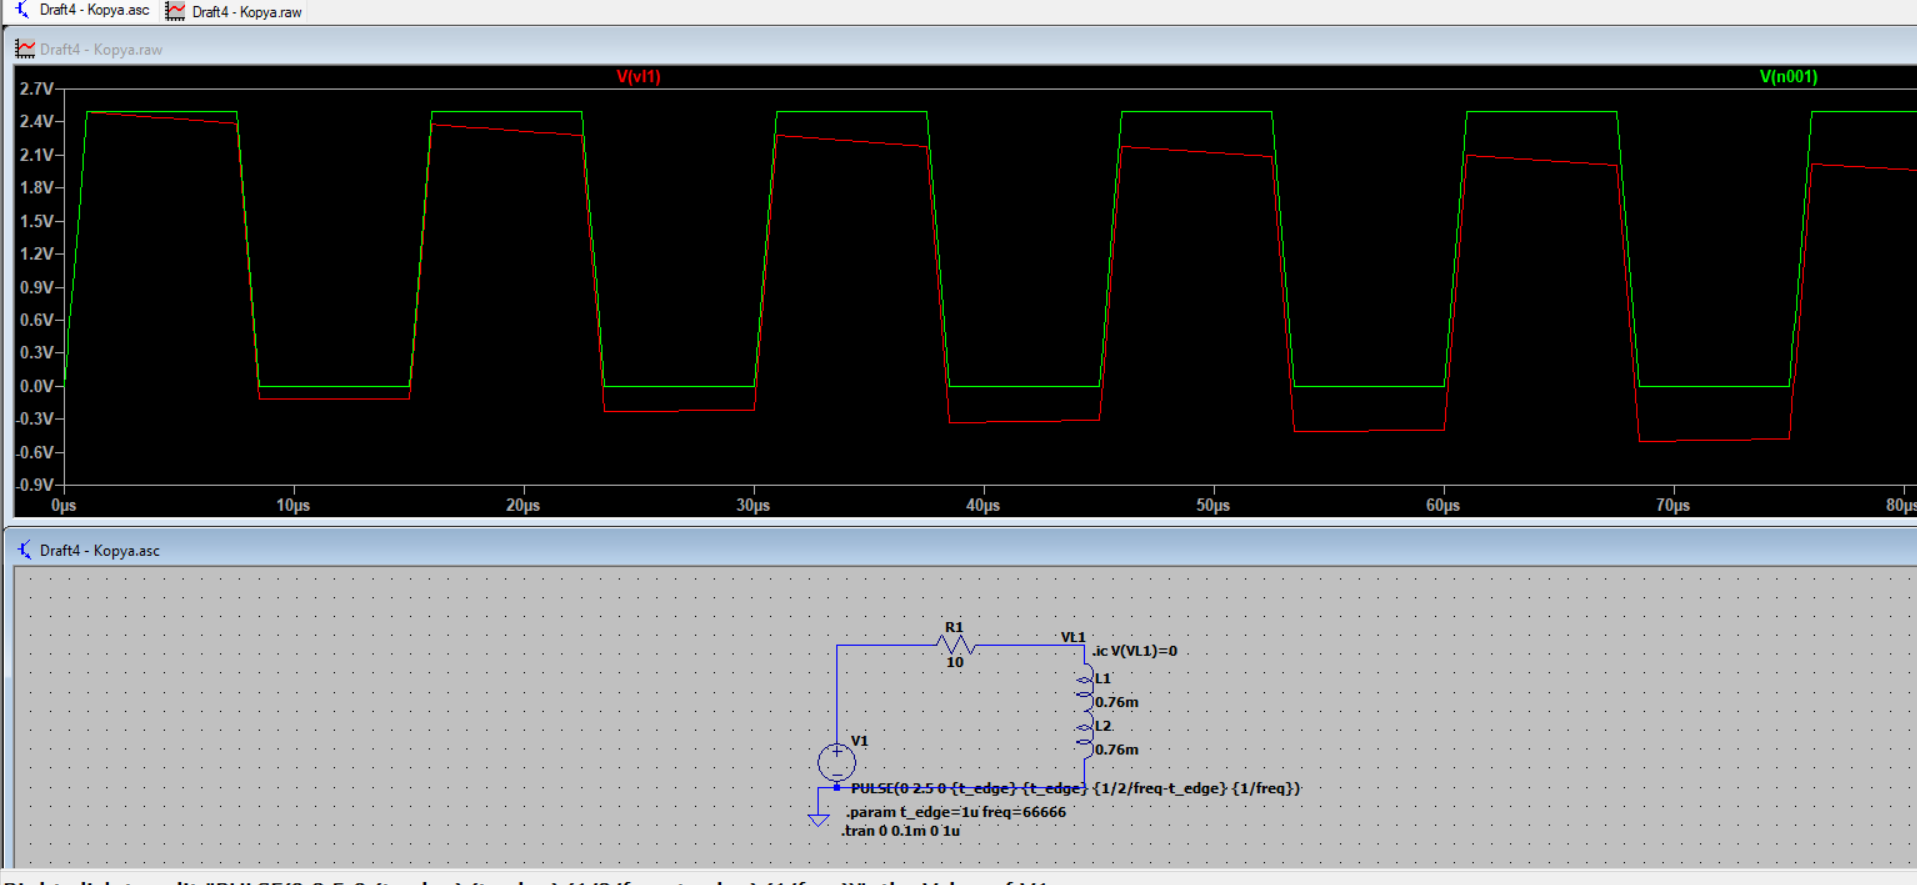
\includegraphics[width=1\textwidth]{assets/66666-hz-2.5vpp-sim.png}
    \caption{66.66kHz Output @ $2.5V_{pp}$}
    \label{fig:6666-hz-2.5vpp-output}
\end{figure}

Same characteristics as the experimental results are observed in the simulation.

\newpage{}
\thispagestyle{plain}

\subsubsection{Reducing the Amplitude}
When the amplitude of the square wave is reduced to half (0-2.5V), the voltages across both the inductor and the resistor also reduce proportionally. The overall behavior and response times remain consistent, but the magnitude of the voltages is halved.

	\chapter{Results and Discussion}

\section{Magnetic Field Analysis}
In a Helmholtz coil configuration, where two identical coils are separated by a distance equal to their radius, the magnetic field between the coils is highly uniform around the midpoint, enhancing precision in experiments requiring consistent magnetic fields.

\section{Inductance Calculation}
We have calculated the inductance of the coil using the formula \( L = \frac{\mu_0 N^2 A}{l} \). The inductance of one coil is calculated \( L = 0.63 \)mH and the inductance of the two coils in series is calculated as \( L = 1.26 \)mH.

\section{Experimental Observations}

The measurement of the inductance of the coil was done using a simple RL circuit. The inductance of the coil was calculated to be 1.53mH. Calculation system is also verified by measuring a known inductor of 1mH.

\section{Waveform Analysis}

\subsection{Period is More Than Time Constant}
The period of the waveform is more than the time constant, which means that the inductor has enough time to charge and discharge fully. The voltage across the inductor shows a complete exponential rise and fall.

\subsection{Period is Equal to Time Constant}
The period of the waveform is equal to the time constant, which means that the inductor has just enough time to charge and discharge fully. The voltage across the inductor shows partial exponential rise and fall

\newpage
\thispagestyle{plain}

\subsection{Period is Less Than Time Constant}
The period of the waveform is less than the time constant, which means that the inductor does not have enough time to charge and discharge fully. The voltage across the inductor barely shows any change

	\chapter{Conclusion}

This project demonstrates the design and analysis of Helmholtz coil to achieve a uniform magnetic field. The theoretical derivations align with the experimental and simulation results, confirming the optimal configuration for uniformity. The study also provides insights into the coil's inductance and behavior in a circuit with varying frequencies and amplitudes.

	\chapter{Appendices}

\section{Data Sheets}

\subsection{Frequency Analysis Data Sheet}

\begin{figure}[h]
    \centering
    \begin{circuitikz} \draw
        (0,0) to[square voltage source, l=0-5V] (0,4)
        to[R, l=$10\Omega$] (4,4) 
        to[L, l=0.76mH] (4,2) 
        to[L, l=0.76mH] (4,0) -- (0,0)
        ;
        \end{circuitikz}
    \caption{Helmholtz Coil Circuit Diagram}
\end{figure}

\subsection{Measurement System Data Sheet}

\begin{figure}[h]
    \centering
    \begin{circuitikz}
        \draw (0,0) to[sinusoidal voltage source, l=$4.16V_{pp}$] (0,4)
        to[R, l=$466\Omega$] (4,4)
        to[L, l=$L_{x}$] (4,0)
        to[short] (0,0);
    \end{circuitikz}
    \caption{Measurement System Circuit Diagram}
\end{figure}

\newpage{}
\thispagestyle{plain}


\subsection{Prototype Board Data Sheet}

\begin{figure}[h]
    \centering
    \begin{circuitikz}
        \tikzstyle{every node}=[font=\normalsize]
        \draw (7.5,8.5) to[R,l={ \normalsize 100$\Omega$}] (7.5,12.25);
        \draw (8.5,12.25) to[R,l={ \normalsize 460$\Omega$}] (8.5,8.5);
        \draw (7.5,8.5) to[short] (8.5,8.5);
        \draw (8,7) to[short] (8,8.5);
        \draw (6.25,12.5) to[short] (9.5,12.5);
        \draw (9.5,12.5) to[short] (9.5,14);
        \draw (9.5,14) to[short] (6.25,14);
        \draw (6.25,14) to[short] (6.25,12.5);
        \draw (7.5,12.25) to[short] (7.5,12.5);
        \draw (8.5,12.25) to[short] (8.5,12.5);
        \node at (7.5,12.5) [circ] {};
        \node at (8.5,12.5) [circ] {};
        \node [font=\small] at (7.75,13.25) {ON-ON SWITCH};
        \draw (13,8.5) to[L,l={ \normalsize 1mH} ] (13,12.5);
        \draw (14.25,12.5) to[L,l={ \normalsize 1.53mH} ] (14.25,8.5);
        \draw (13,8.5) to[short] (14.25,8.5);
        \node at (8,14) [circ] {};
        \draw (13,12.5) to[short] (14.25,12.5);
        \draw (8,14) to[short] (8,14.25);
        \draw (8,14.25) to[short] (13.75,14.25);
        \draw (13.75,14.25) to[short] (13.75,12.5);
        \draw (12.25,8.5) to[short] (15,8.5);
        \node [font=\small] at (13.5,7.75) {ON-ON SWITCH};
        \draw (12.25,8.5) to[short] (12,8.5);
        \draw (12,8.5) to[short] (12,7);
        \draw (12,7) to[short] (15,7);
        \draw (15,7) to[short] (15,8.5);
        \node at (13,8.5) [circ] {};
        \node at (14.25,8.5) [circ] {};
        \node at (13.5,7) [circ] {};
        \draw (9.5,6.25) to[sinusoidal voltage source, sources/symbol/rotate=auto] (11.75,6.25);
        \draw (9.5,6.25) to[short] (8,6.25);
        \draw (8,6.25) to[short] (8,7);
        \draw (11.75,6.25) to[short] (13.5,6.25);
        \draw (13.5,6.25) to[short] (13.5,7);
    \end{circuitikz}
    \caption{Prototype Board Data Sheet}
\end{figure}

\section{LTspice Netlist}

\begin{lstlisting}
* Helmholtz Coil Simulation
V1 N001 0 PULSE(0 5 0 {t_edge} {t_edge} {1/2/freq-t_edge} {1/freq})
R1 VL1 N001 10
L1 VL1 P001 0.76m
L2 P001 0 0.76m
.tran 0 10m 0 1u
.param t_edge=1u freq=666
.ic V(VL1)=0
.backanno
.end
\end{lstlisting}


	\newpage
	\thispagestyle{plain}
	\printbibliography{}
\end{document}
